\documentclass[11pt]{beamer}
\usetheme{Pittsburgh}
\usepackage[utf8]{inputenc}
\usepackage[english]{babel}
\usepackage{amsmath}
\usepackage{amsfonts}
\usepackage{amssymb}
\usepackage{graphicx}
\usepackage{proof}
\usepackage{tikz}
\usepackage{url}

% add slide numbering
\addtobeamertemplate{navigation symbols}{}{%
    \usebeamerfont{footline}%
    \usebeamercolor[fg]{footline}%
    \hspace{1em}%
    \insertframenumber/\inserttotalframenumber
}

\author{Vincent Loup}
\title{Reconsidering generic composition}
\institute{EPFL} 
\date{May 29, 2017} 

\begin{document}

\begin{frame}
\titlepage
\end{frame}

\begin{frame}{Table of contents}
\tableofcontents
\end{frame}

\section{Introduction}
\begin{frame}{Introduction}
We want to ensure messages are unaltered and confidential.

\begin{center}
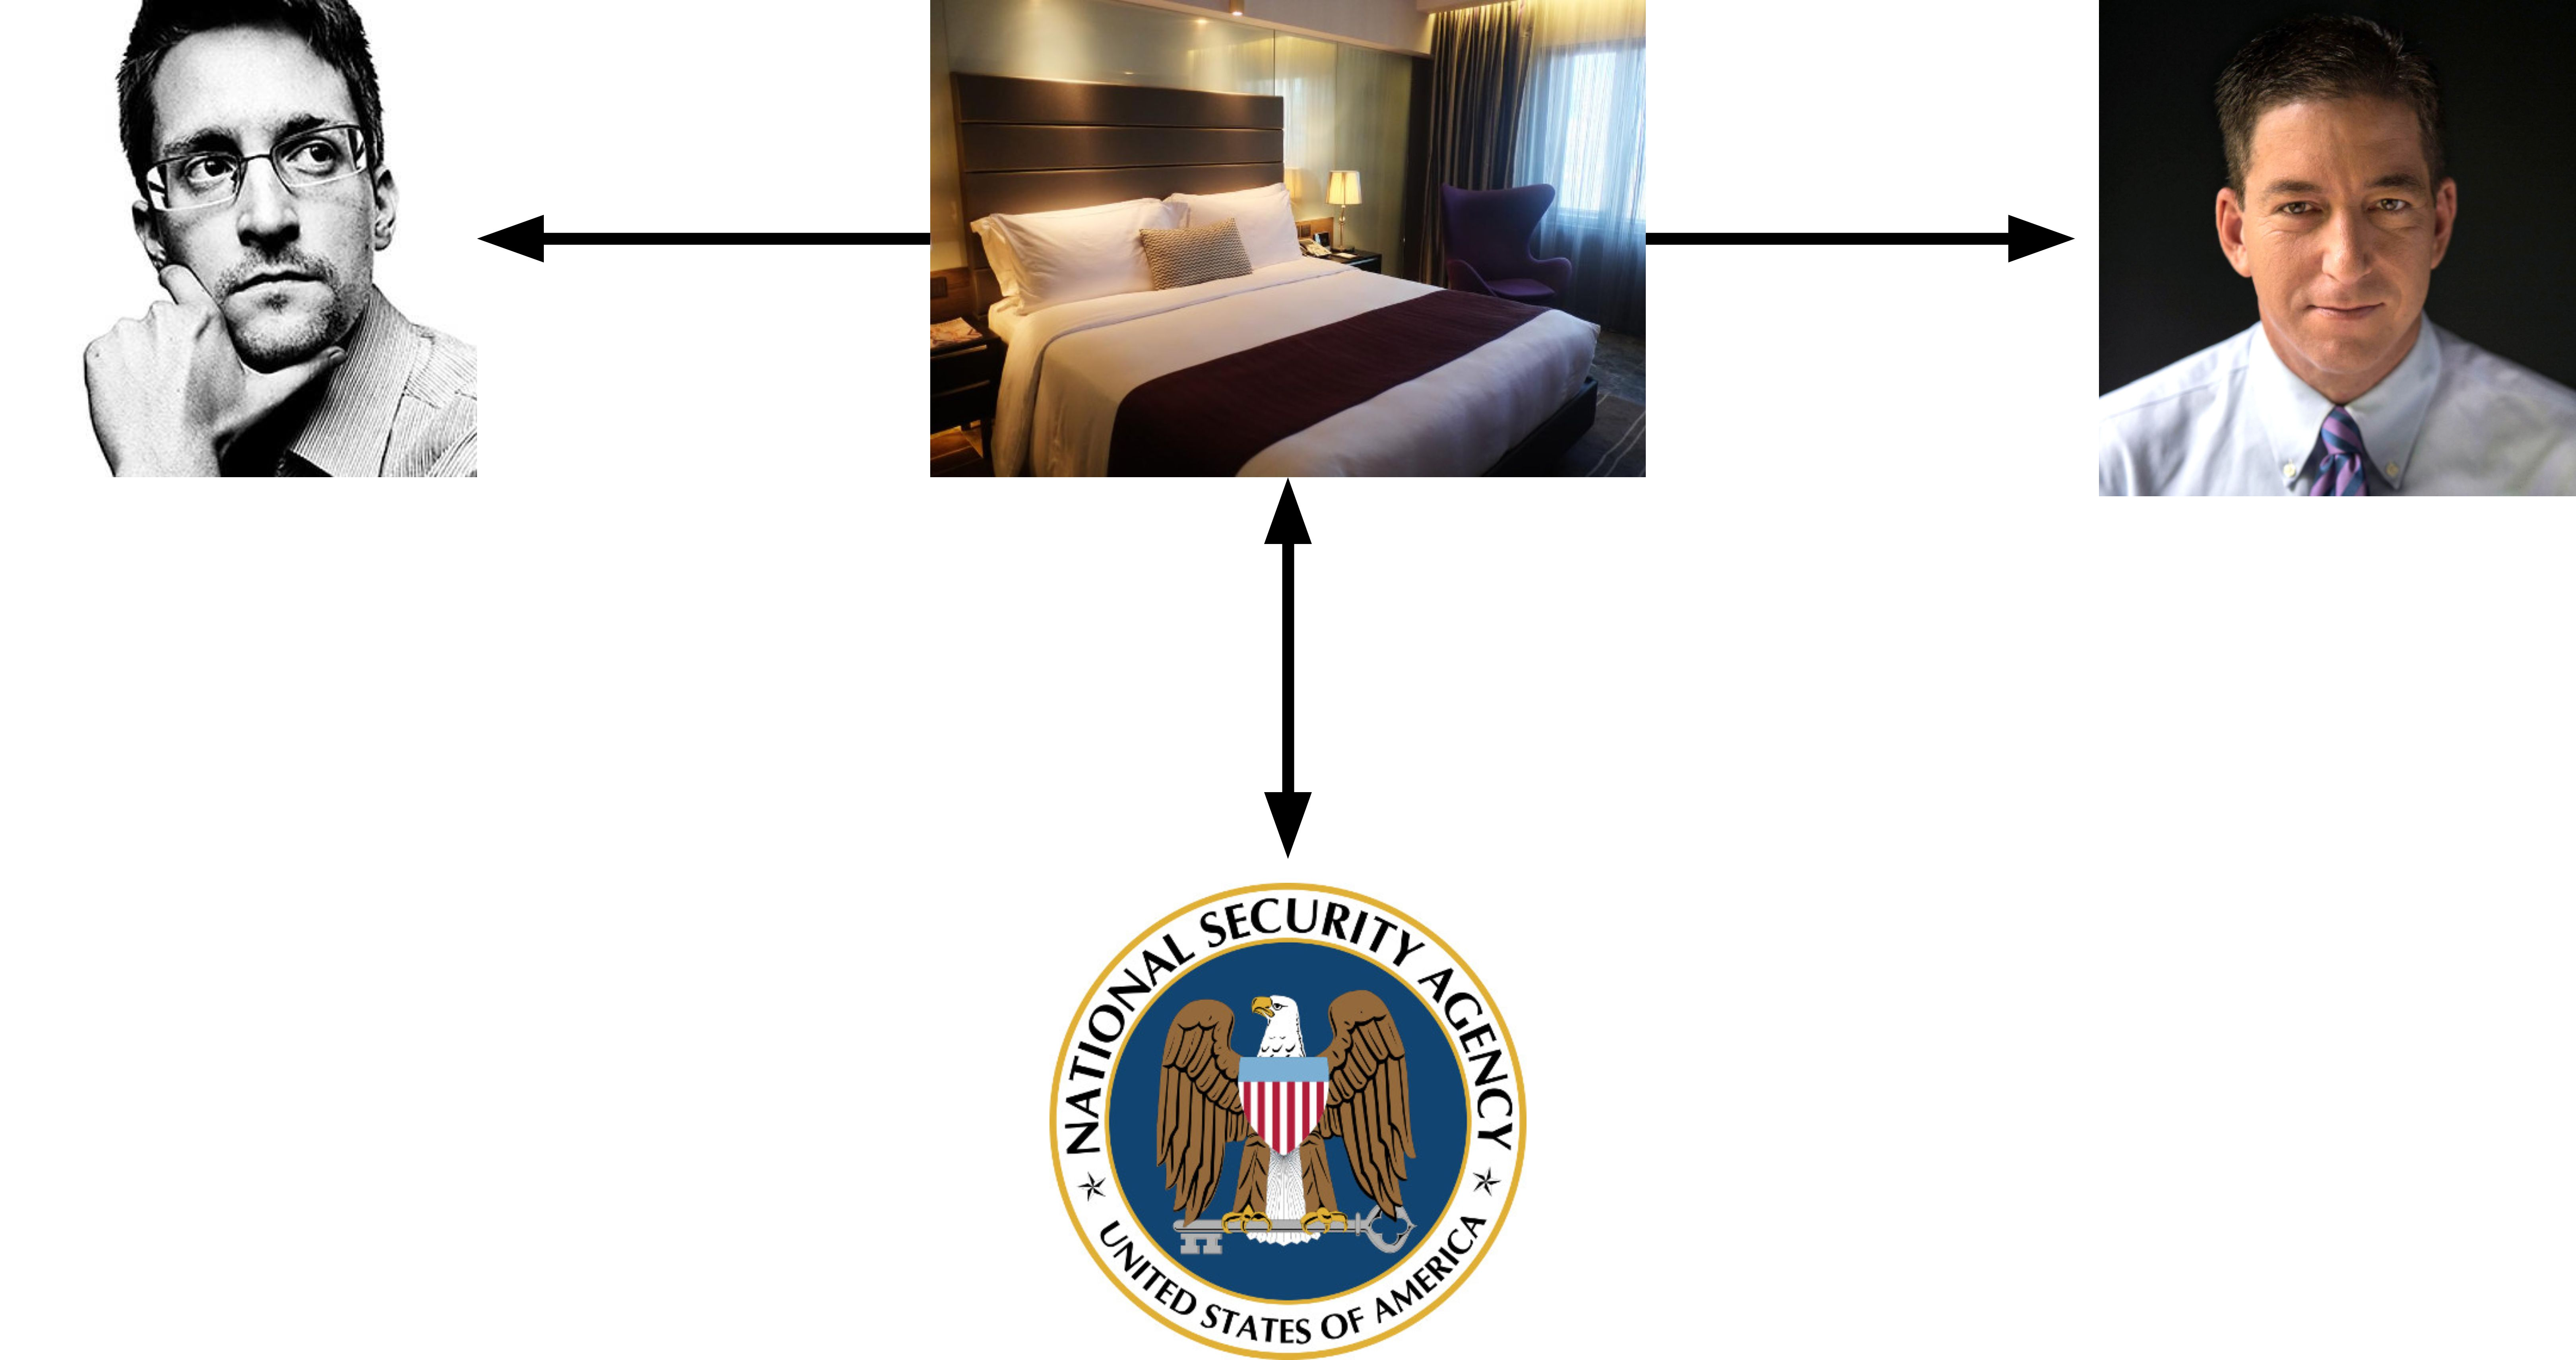
\includegraphics[scale=0.04]{alicebob.jpg}
\end{center}

Authenticated encryption is the solution to this problem.
\end{frame}

\begin{frame}{Authenticated Encryption (AE)}
AE provides
\begin{itemize}
\item Confidentiality
\item Integrity
\item Authentication
\end{itemize}

Generic composition: construction of Authenticated Encryption with an encryption scheme and a MAC.

Dedicated schemes: CCM, GCM or the ongoing CAESAR competition also provide authenticated encryption.
\end{frame}

\section{Generic composition}
\begin{frame}{Generic composition}
\begin{itemize}
\item Combine a MAC and an encryption scheme together as black boxes.
\item Uses off the shelves schemes.
\item First results in 2000, problem revisited in 2014.
\end{itemize}
\end{frame}

\begin{frame}{Probabilistic schemes}
First results of 2000 assumes we have probabilistic schemes.

\begin{center}
\begin{tabular}{ c c }
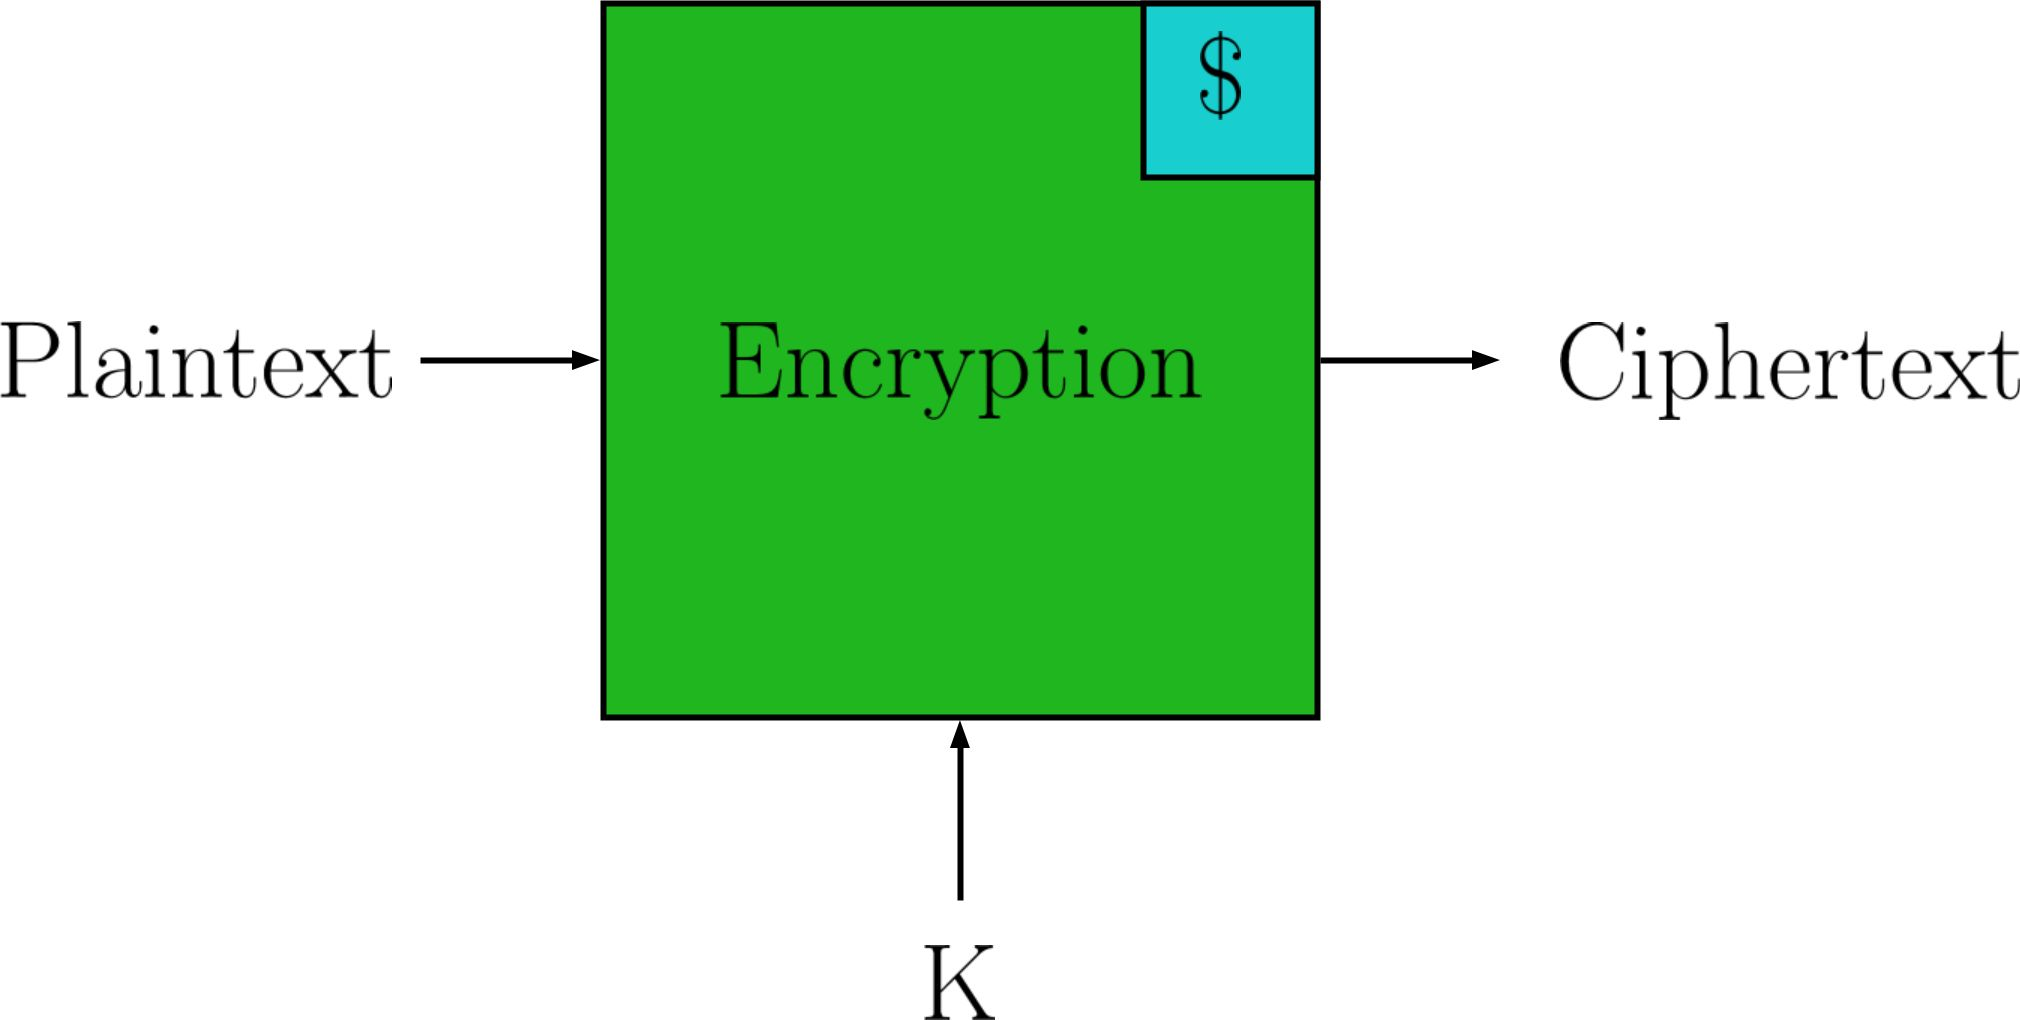
\includegraphics[scale=0.08]{probEnc.jpg} & 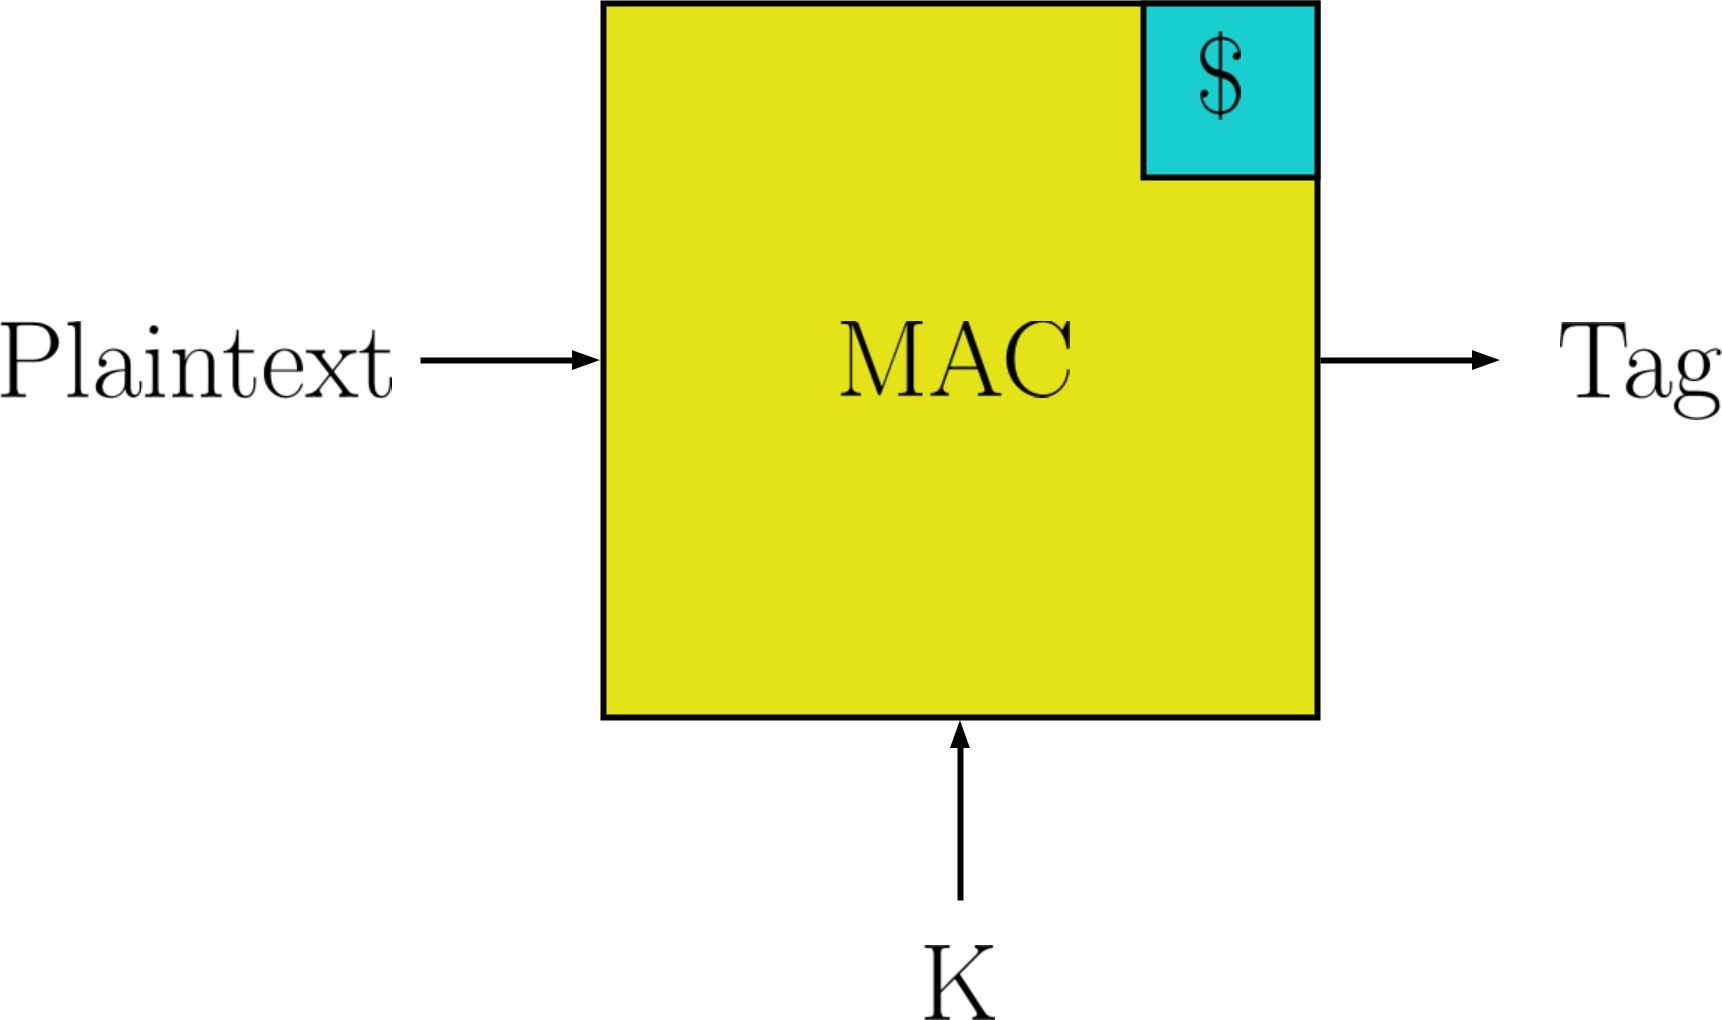
\includegraphics[scale=0.08]{probMac.jpg} \\
	$E(K_e, M) = C$ & $T(K_m, M) = Tag$
\end{tabular}
\end{center}
\end{frame}

\begin{frame}{Encrypt-and-MAC (E\&M)}
$\overline{E}(K_e||K_m, M) = E(K_e,M)||T(K_m, M)$

\begin{center}
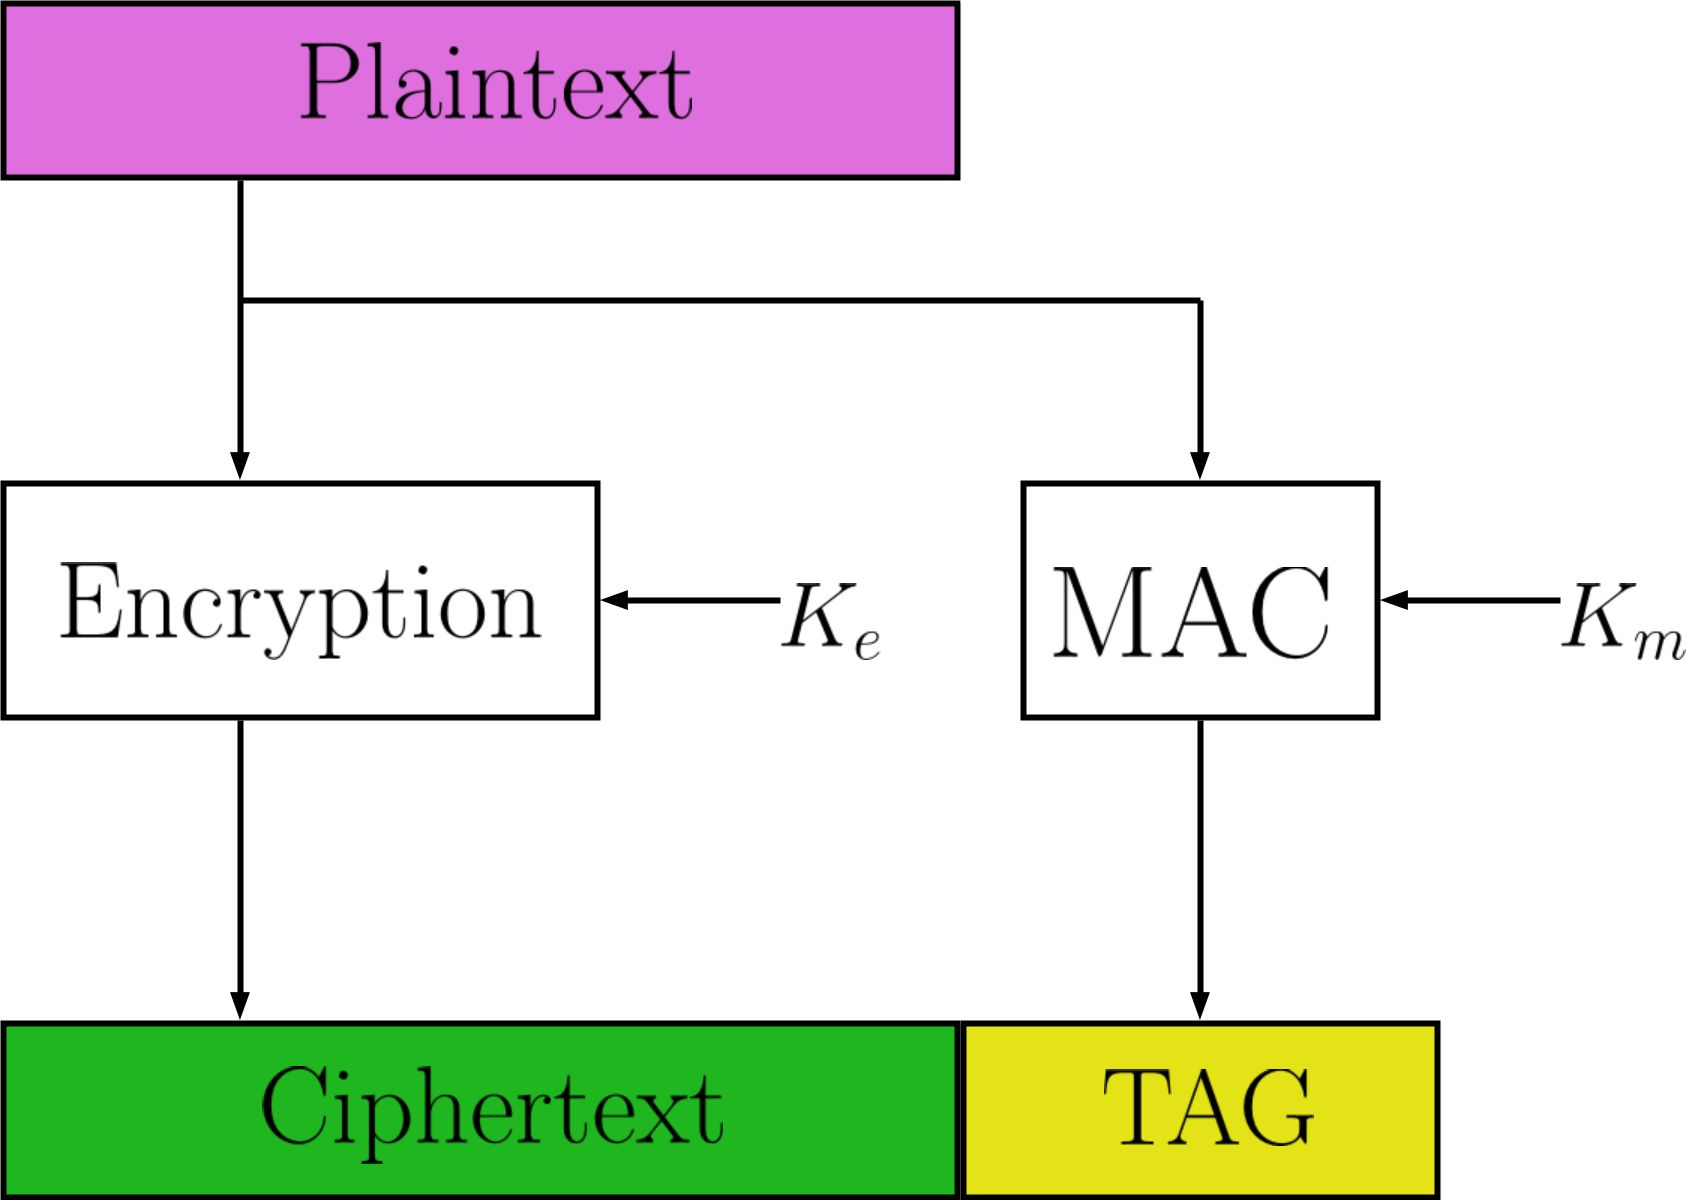
\includegraphics[scale=0.1]{EandM.jpg}
\end{center}

We can compute $E(K_e, M)$ and $T(K_m, M)$ in parallel.

The SSH protocol is implementing this construction.

\end{frame}

\begin{frame}{MAC-then-Encrypt (MtE)}
$\overline{E}(K_e||K_m, M) = E(K_e,M||T(K_m, M))$

\begin{center}
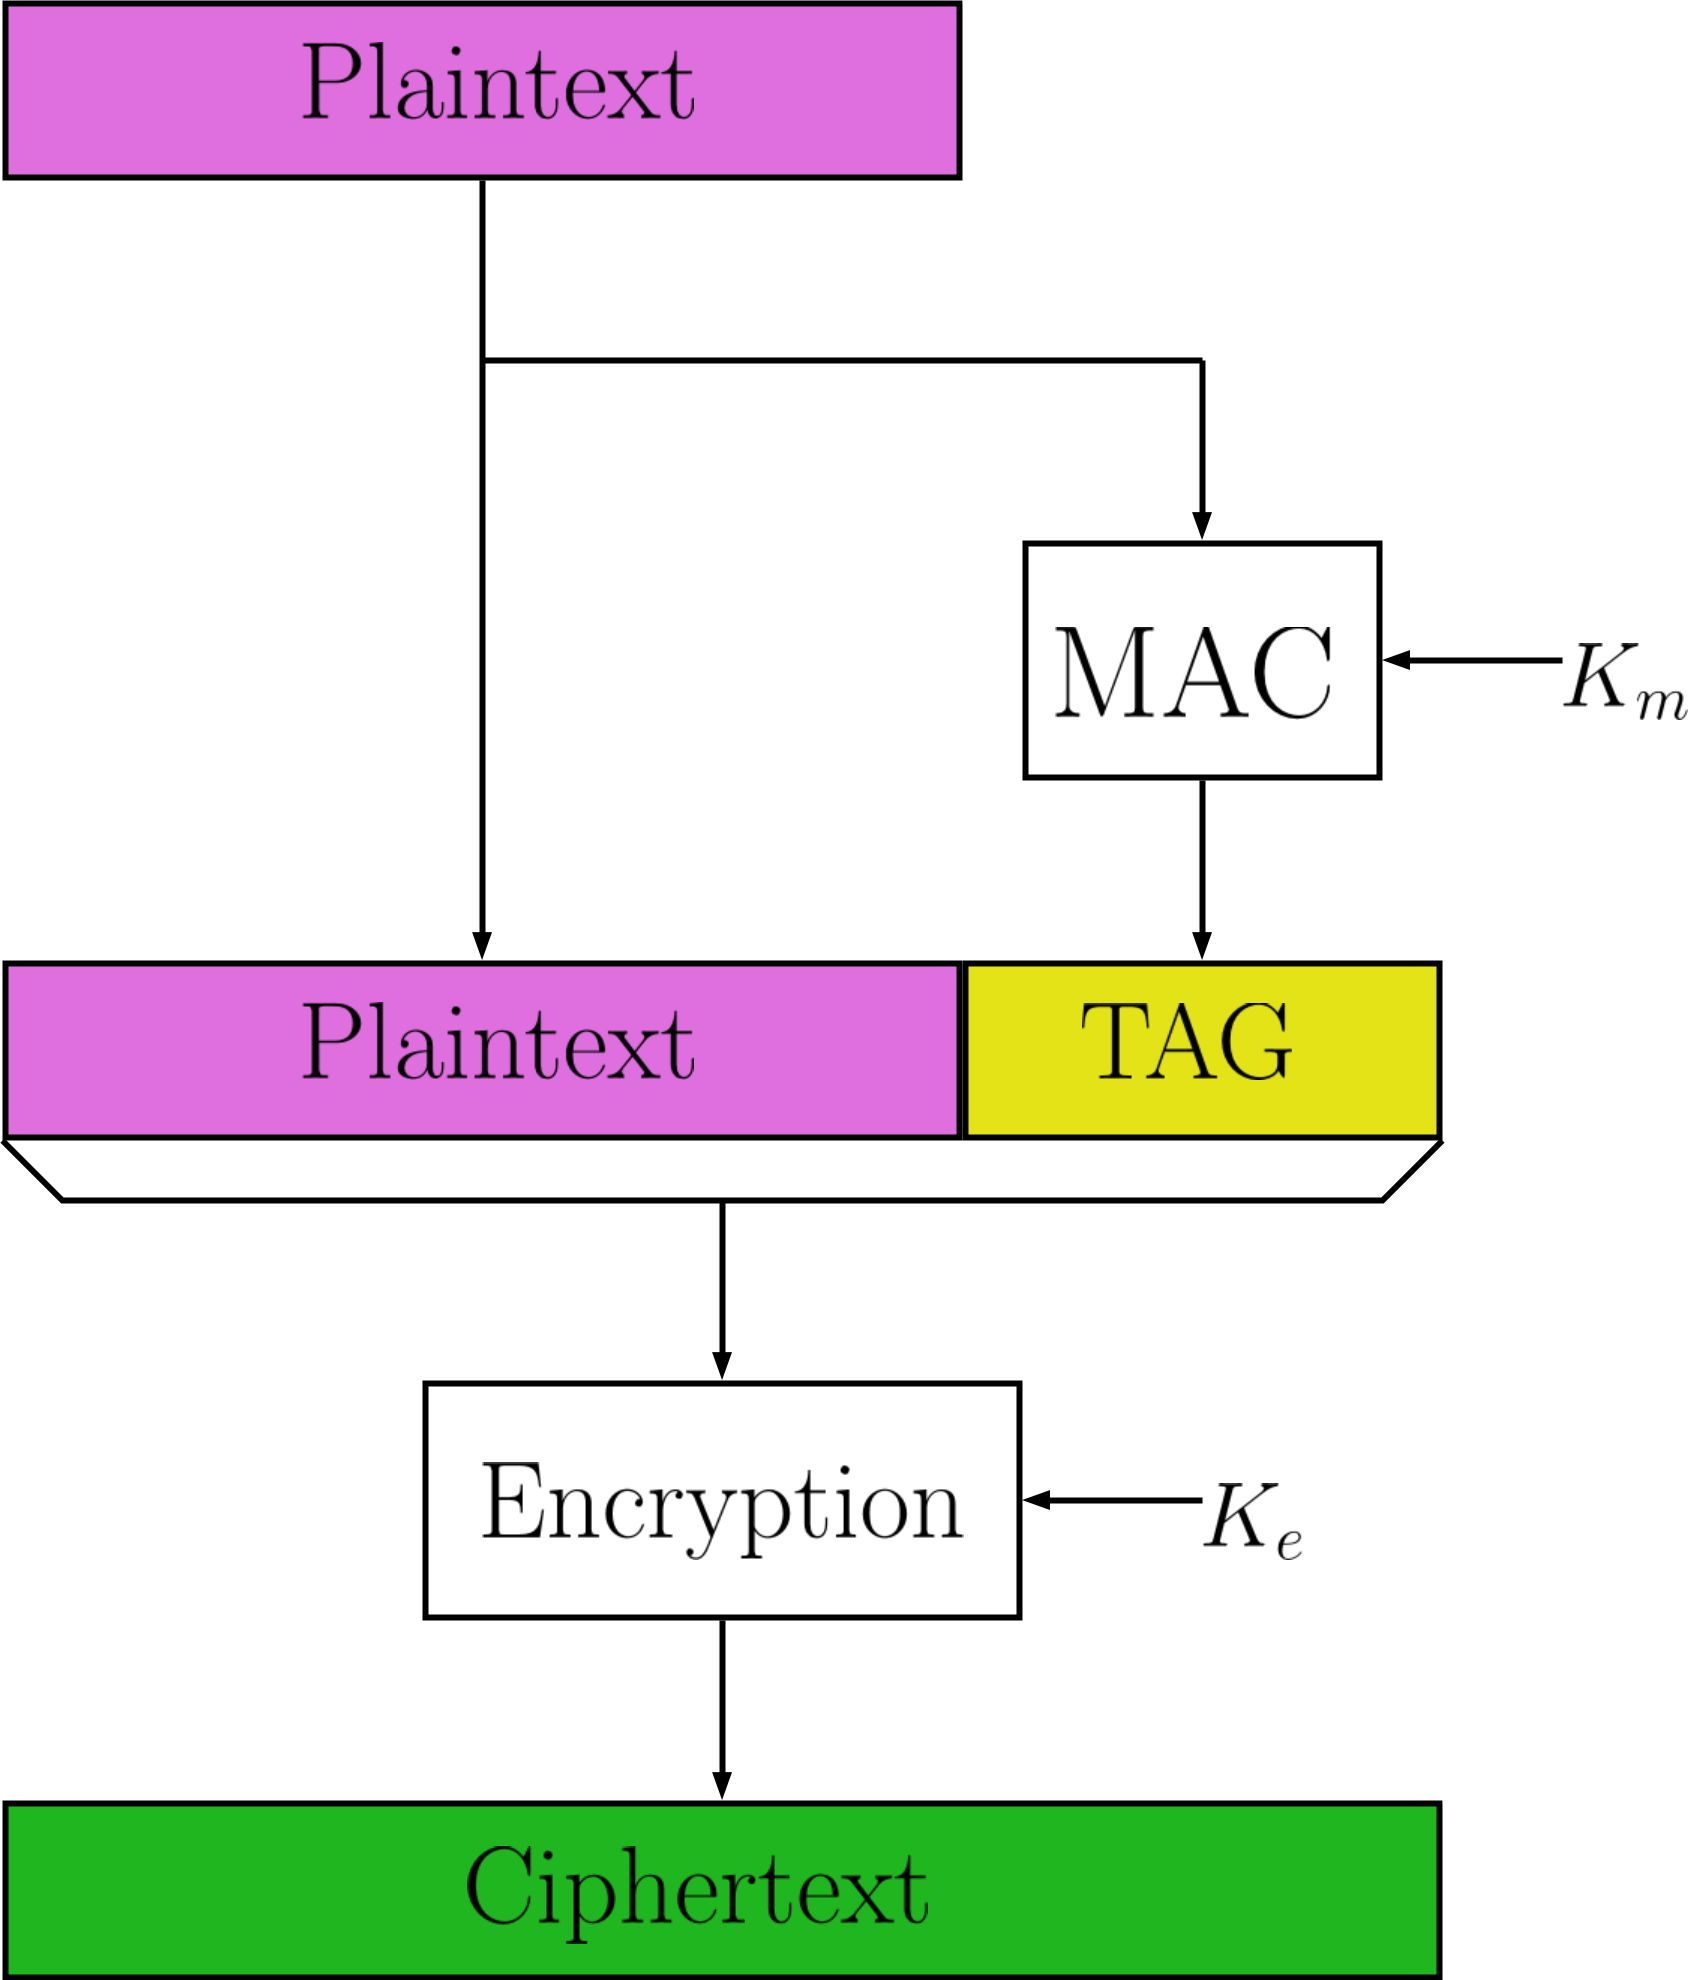
\includegraphics[scale=0.07]{MthenE.jpg}
\end{center}

The MAC is encrypted, so harder to attack.

SSL/TLS is implementing this construction.
\end{frame}

\begin{frame}{Encrypt-then-MAC (EtM)}
$\overline{E}(K_e||K_m, M) = C||T(K_m,C)$ where $C = E(K_e, M)$

\begin{center}
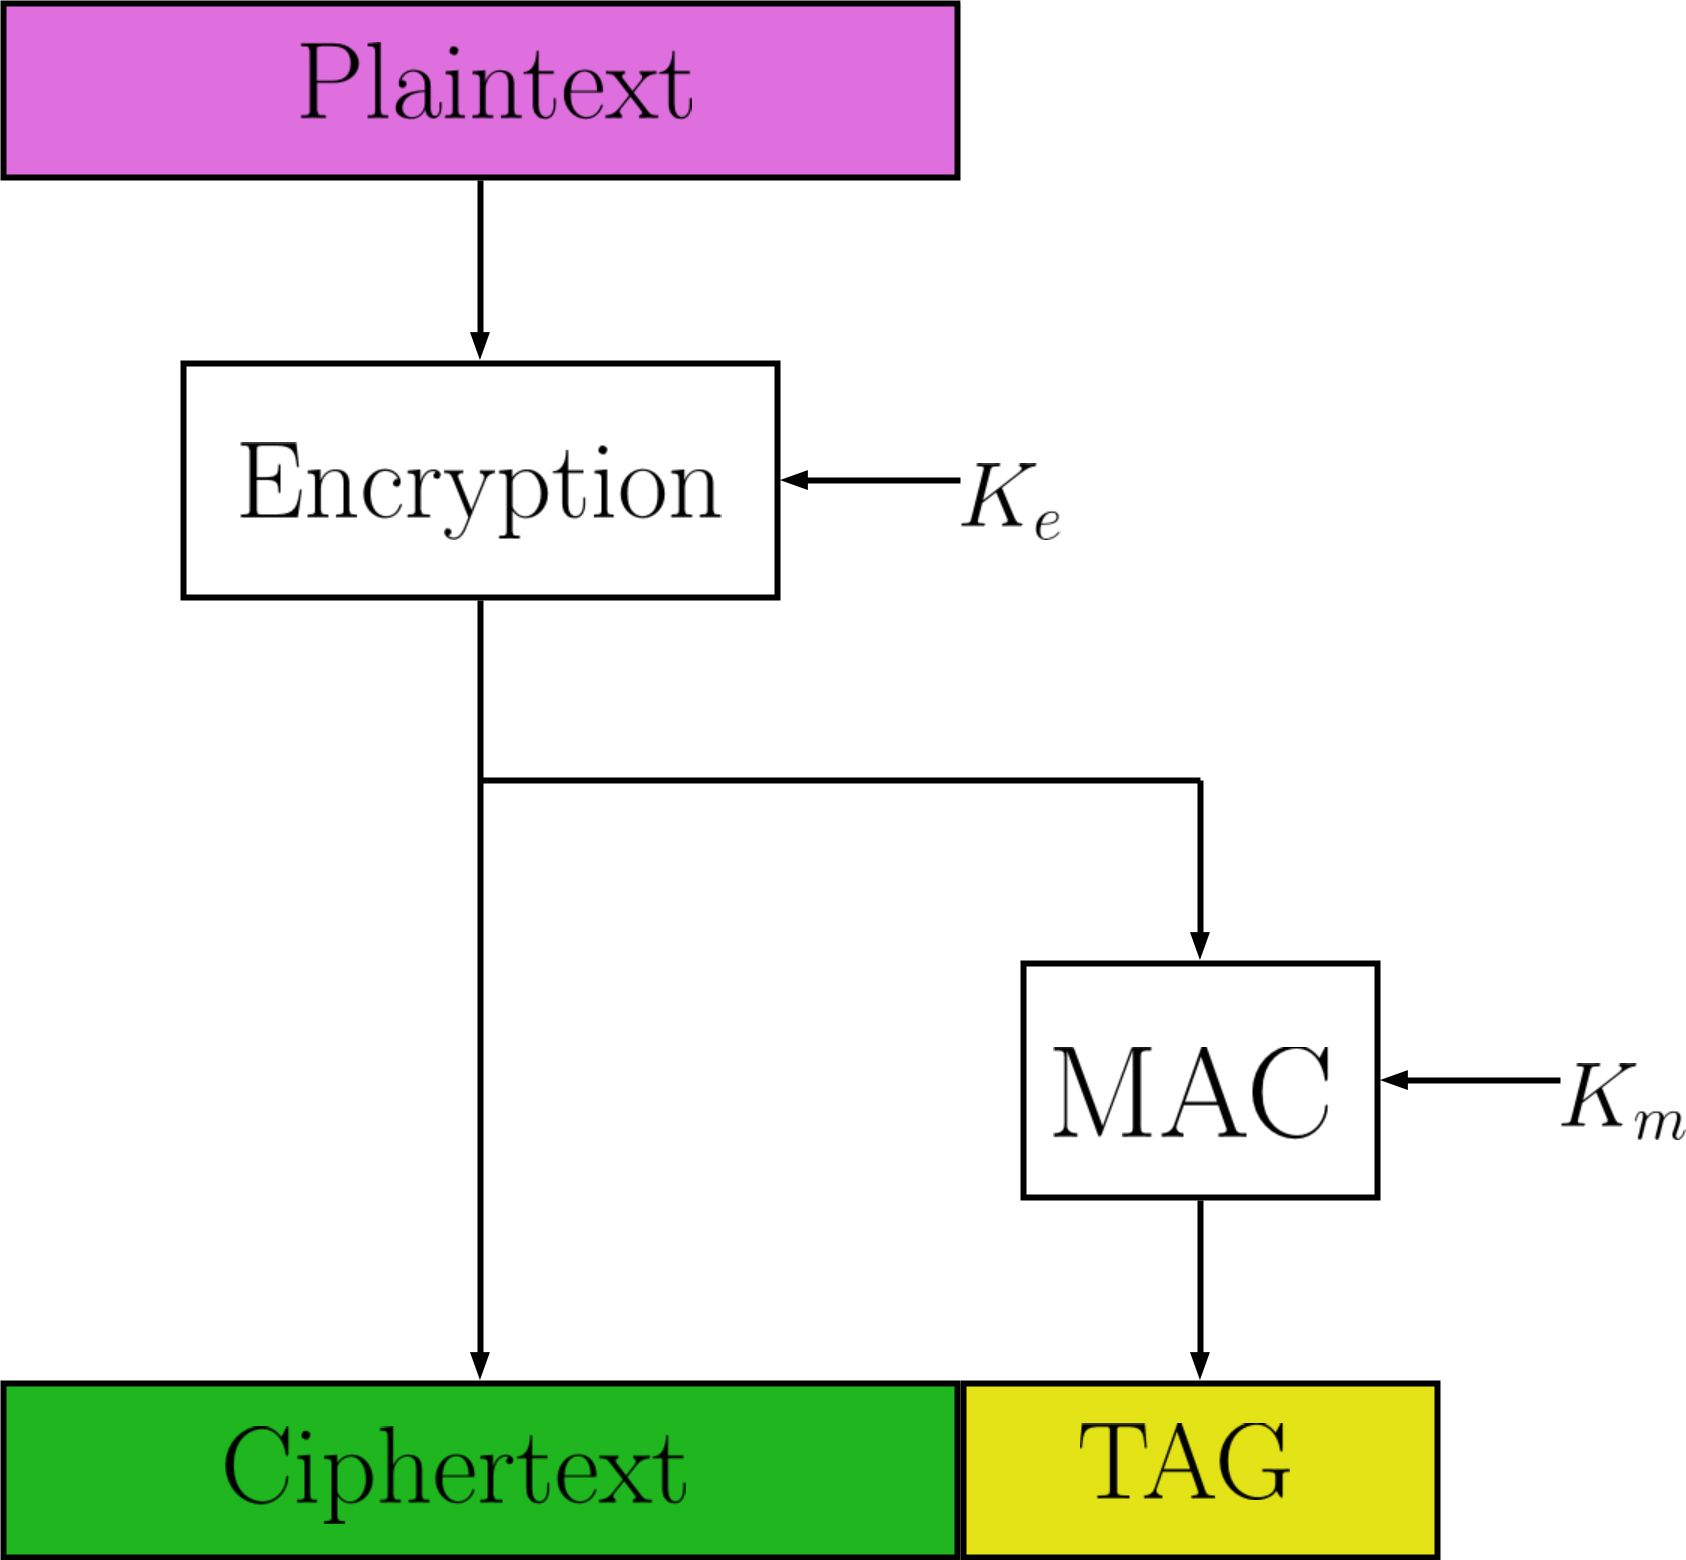
\includegraphics[scale=0.1]{EthenM.jpg}
\end{center}

We calculate the MAC of the ciphertext, not the plaintext.

EtM is implemented in IPSec.
\end{frame}

\begin{frame}{Security of M\&E, MtE and EtM}
\framesubtitle{Bellare and Namprempre, 2000}
\begin{itemize}
	\item M\&E: MAC can leak information about the message.
	\item MtE: We can create a new valid ciphertext if the encryption is malleable.
	\item EtM: Proven secure if the encryption and the MAC are secure.
\end{itemize}
\end{frame}

\section{Issue of the generic composition}
\begin{frame}{Is that the end?}
Real schemes do not match.
We use a nonce or an initialization vector (IV) external to the schemes.

\begin{center}
\begin{tabular}{ c c }
	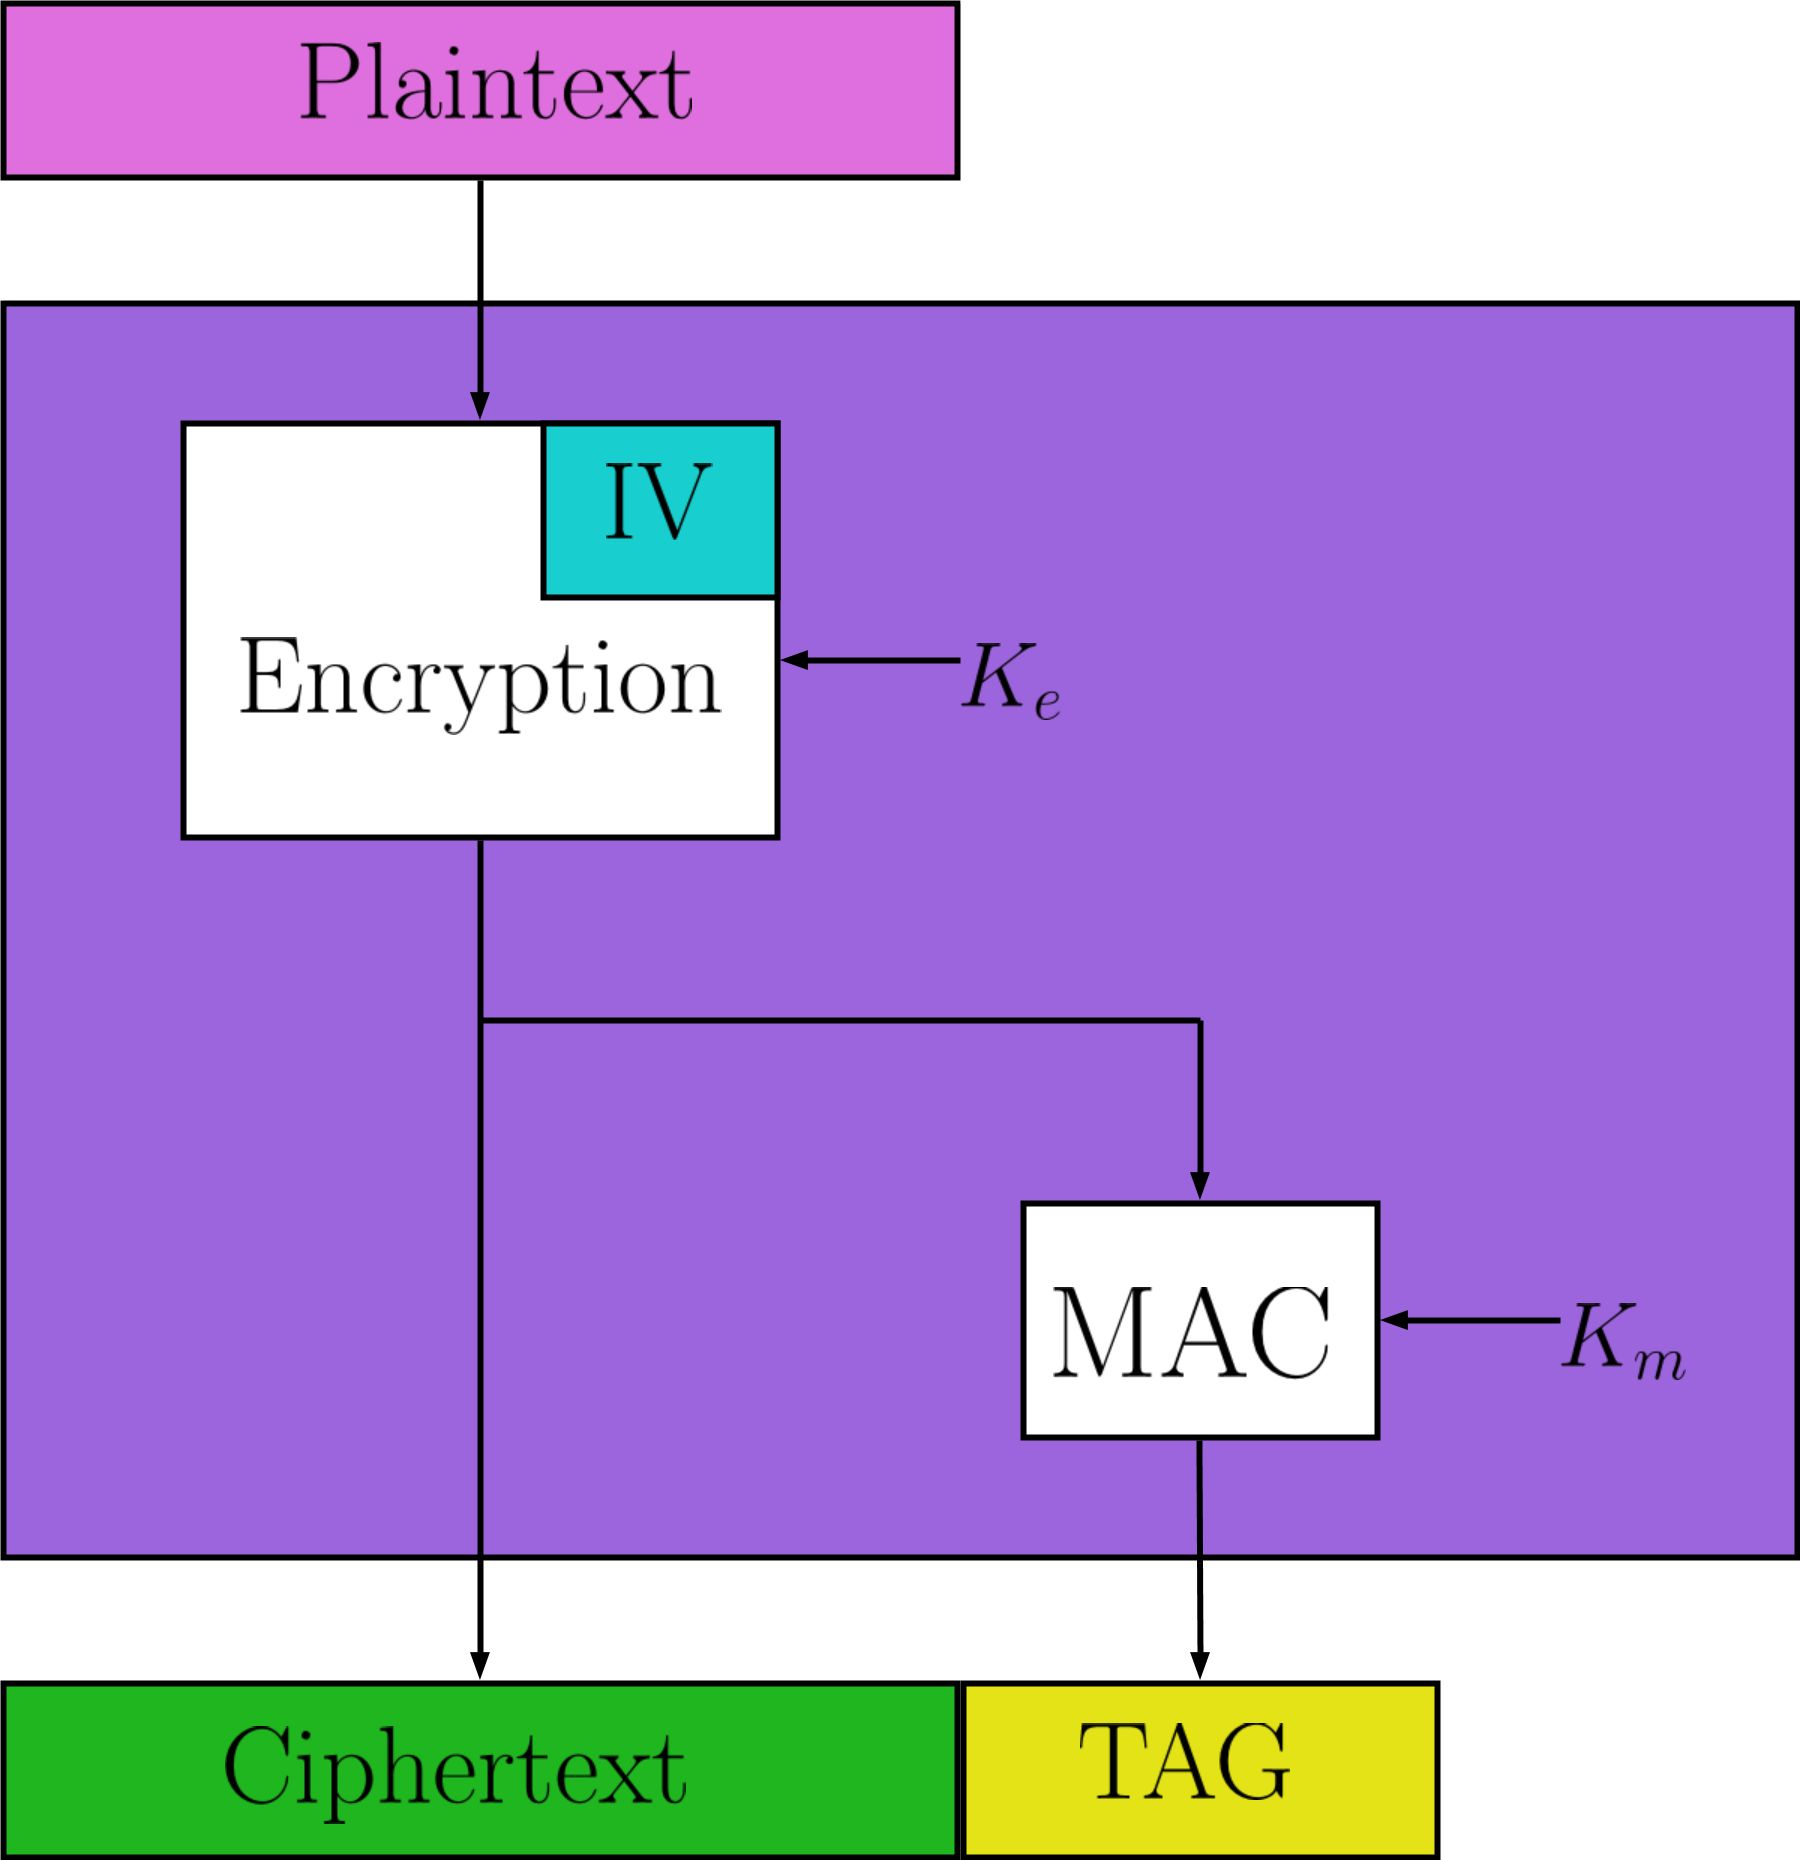
\includegraphics[scale=0.07]{IVThought.jpg} & 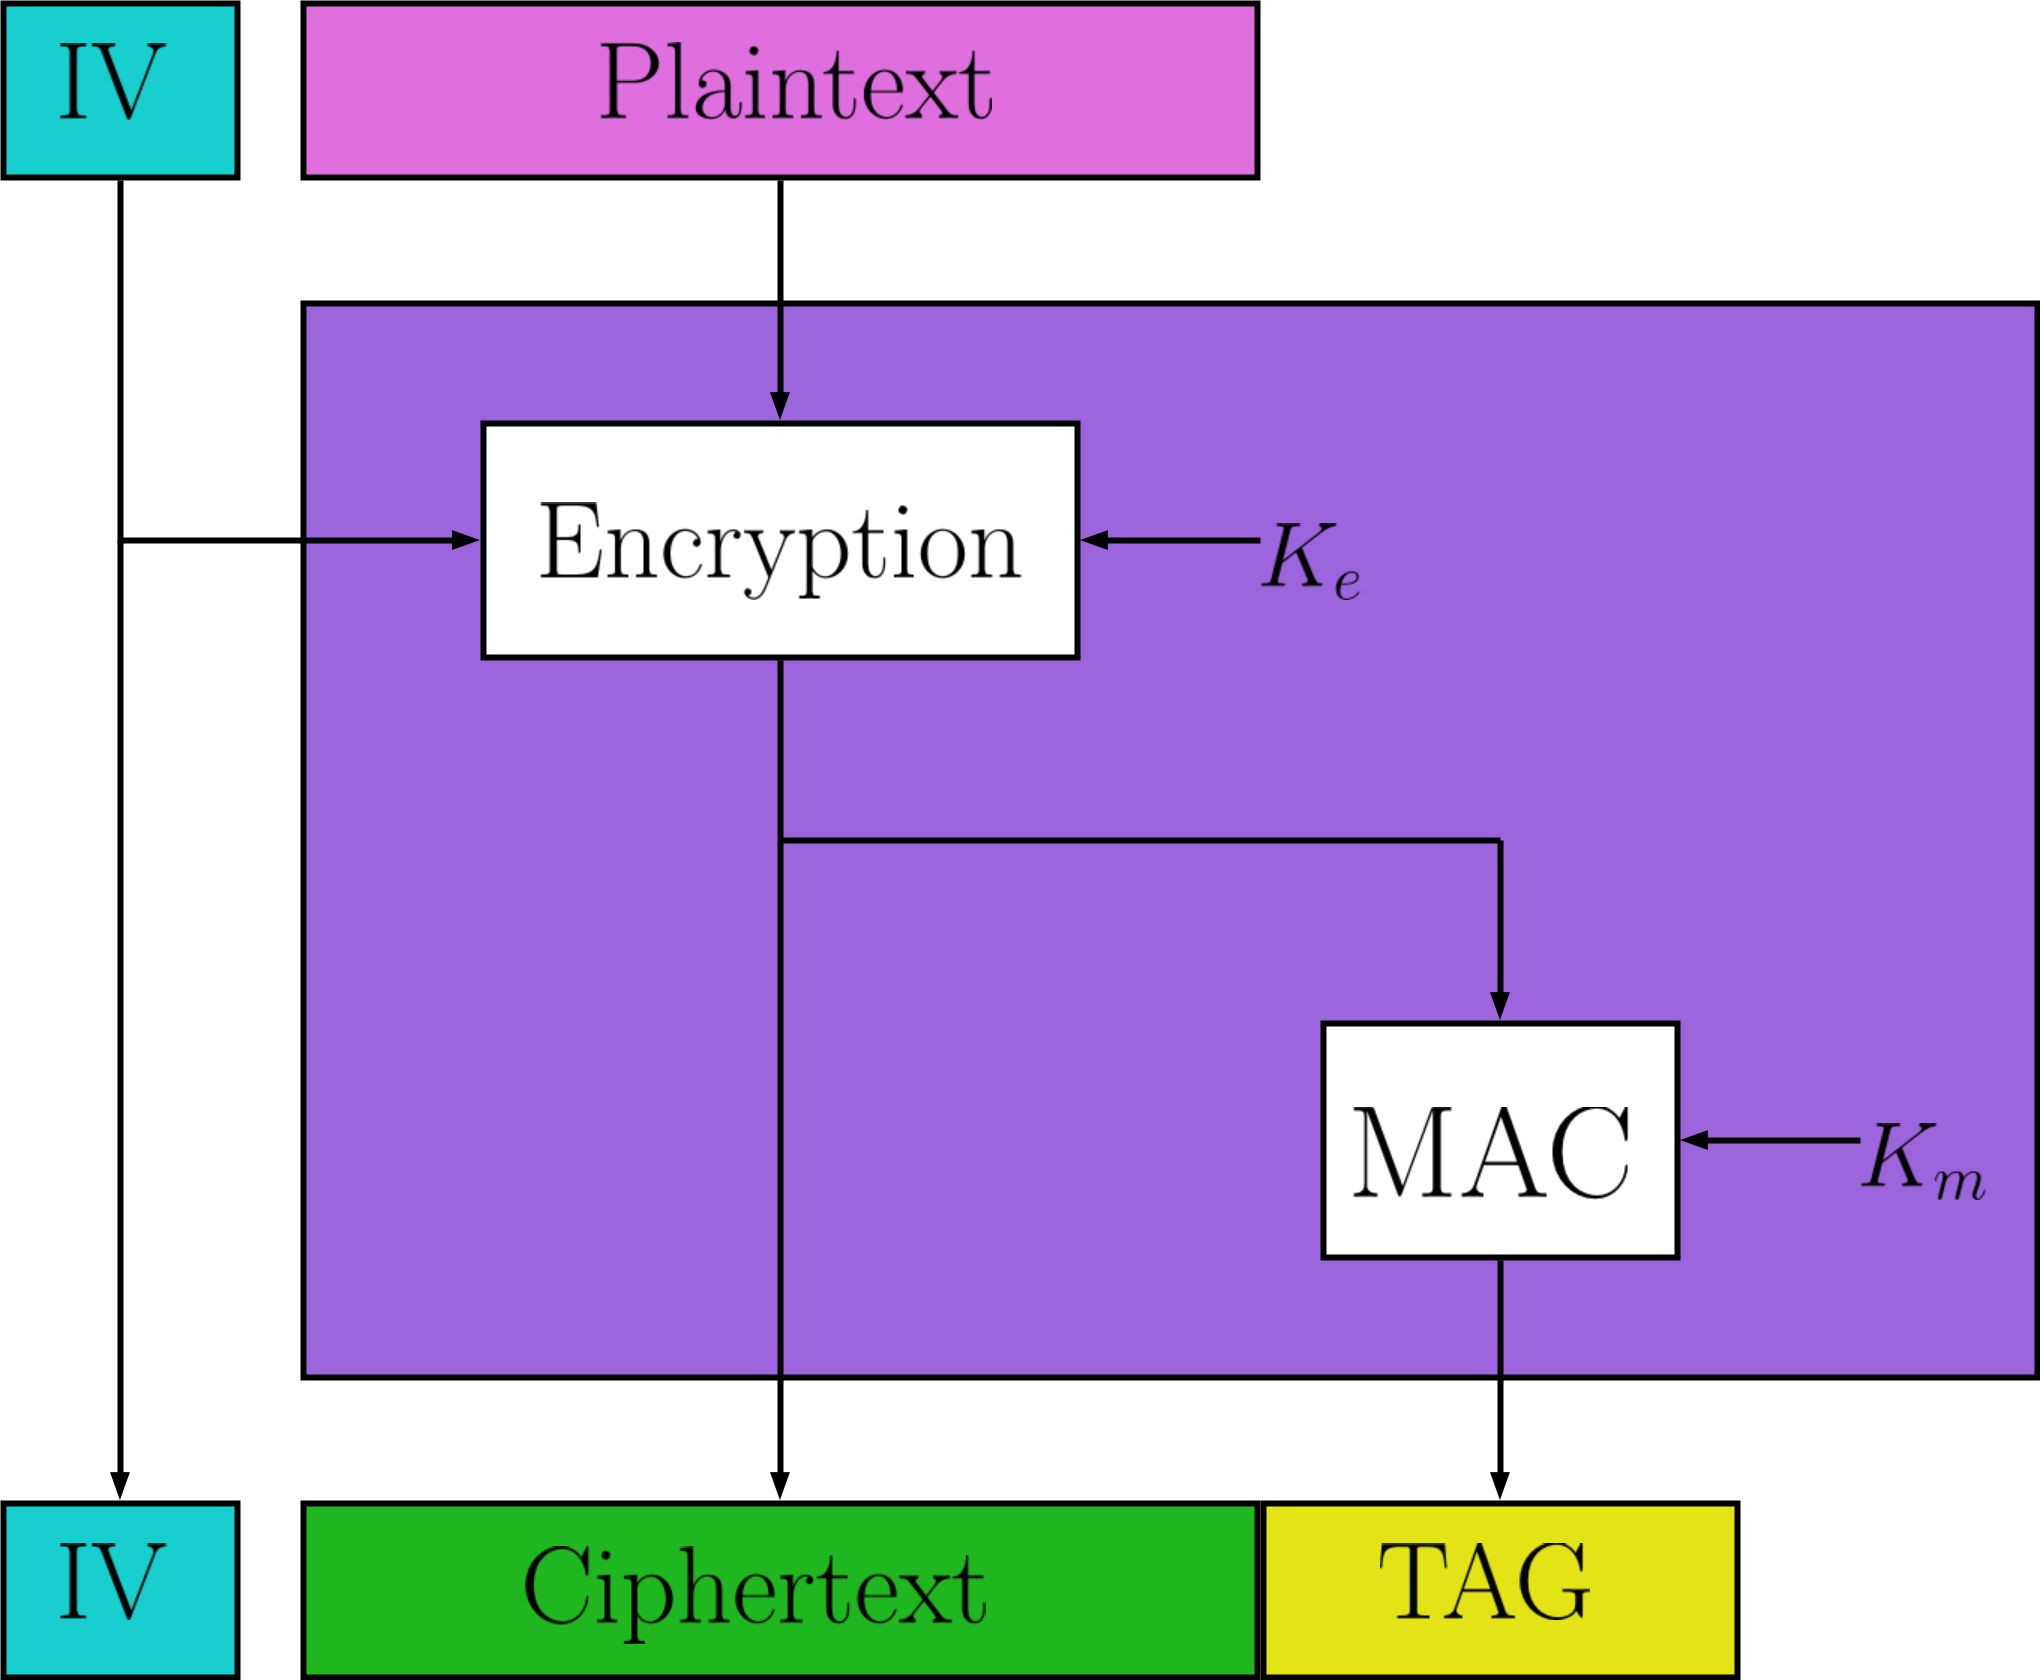
\includegraphics[scale=0.07]{IVBad.jpg}
\end{tabular}
\end{center}
\end{frame}

\section{Reconsidering generic composition}
\begin{frame}{nAE scheme}
$E^{N,A}_K(M) = C$ and $D^{N,A}_K(C) = M$ or $\bot$.

\begin{center}
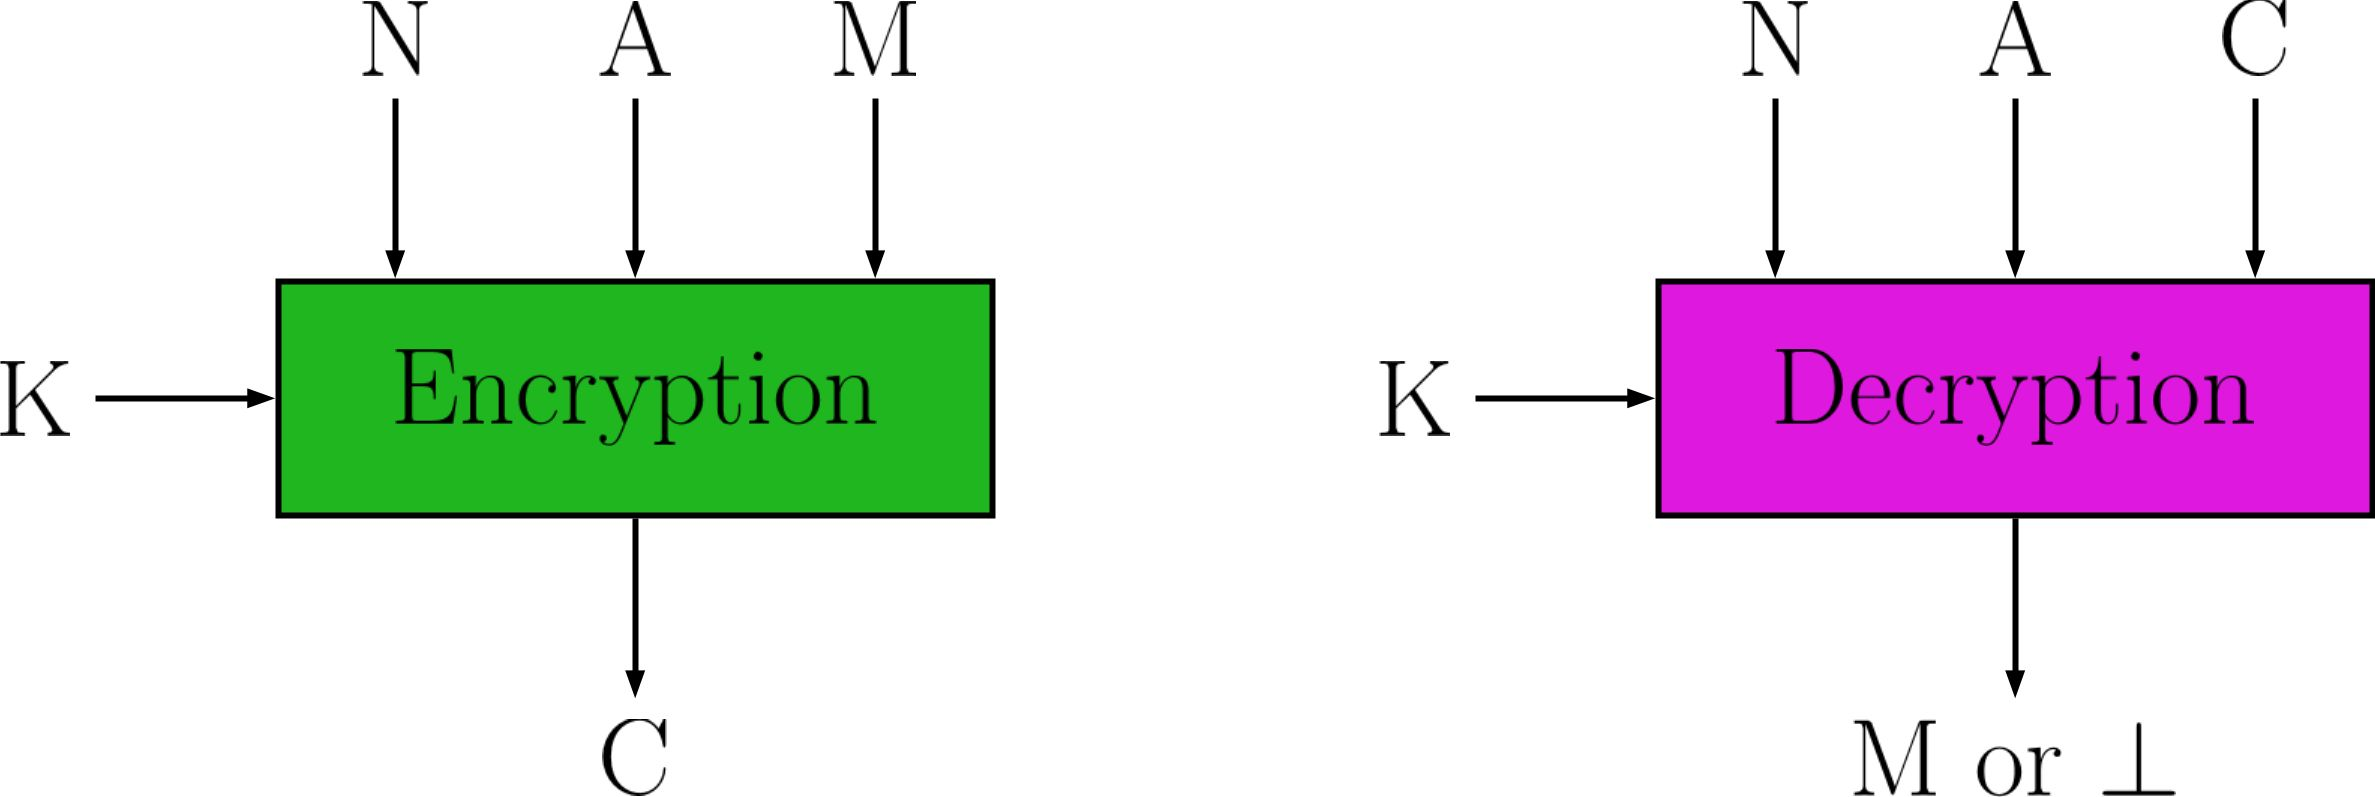
\includegraphics[scale=0.12]{nae.jpg}
\end{center}

N: Nonce

A: Associated data

K: Secret key

M: Message

C: Ciphertext
\end{frame}

\begin{frame}{nAE properties}
Required properties:
\begin{itemize}
\item Correctness: if $E^{N,A}_K(M) = C \not= \bot$ then $D^{N,A}_K(C)=M$
\item Tidiness: if $D^{N,A}_K(C) = M \not= \bot$ then $E^{N,A}_K(M)=C$
\end{itemize}
Security properties:
\begin{itemize}
\item The encryption output is indistinguishable from random strings in a chosen plaintext attack, the adversary must not repeat nonces.
\item The adversary is unable to produce a new valid ciphertext given an encryption oracle. Again, the adversary must not repeat nonces.
\end{itemize}
\end{frame}

\begin{frame}{nE and ivE}
Encryption can be either nonce-based (nE) or IV-based (ivE).

\begin{itemize}
\item IV: random initialization vector.
\item Nonce: unique initialization vector.
\end{itemize}
\begin{center}
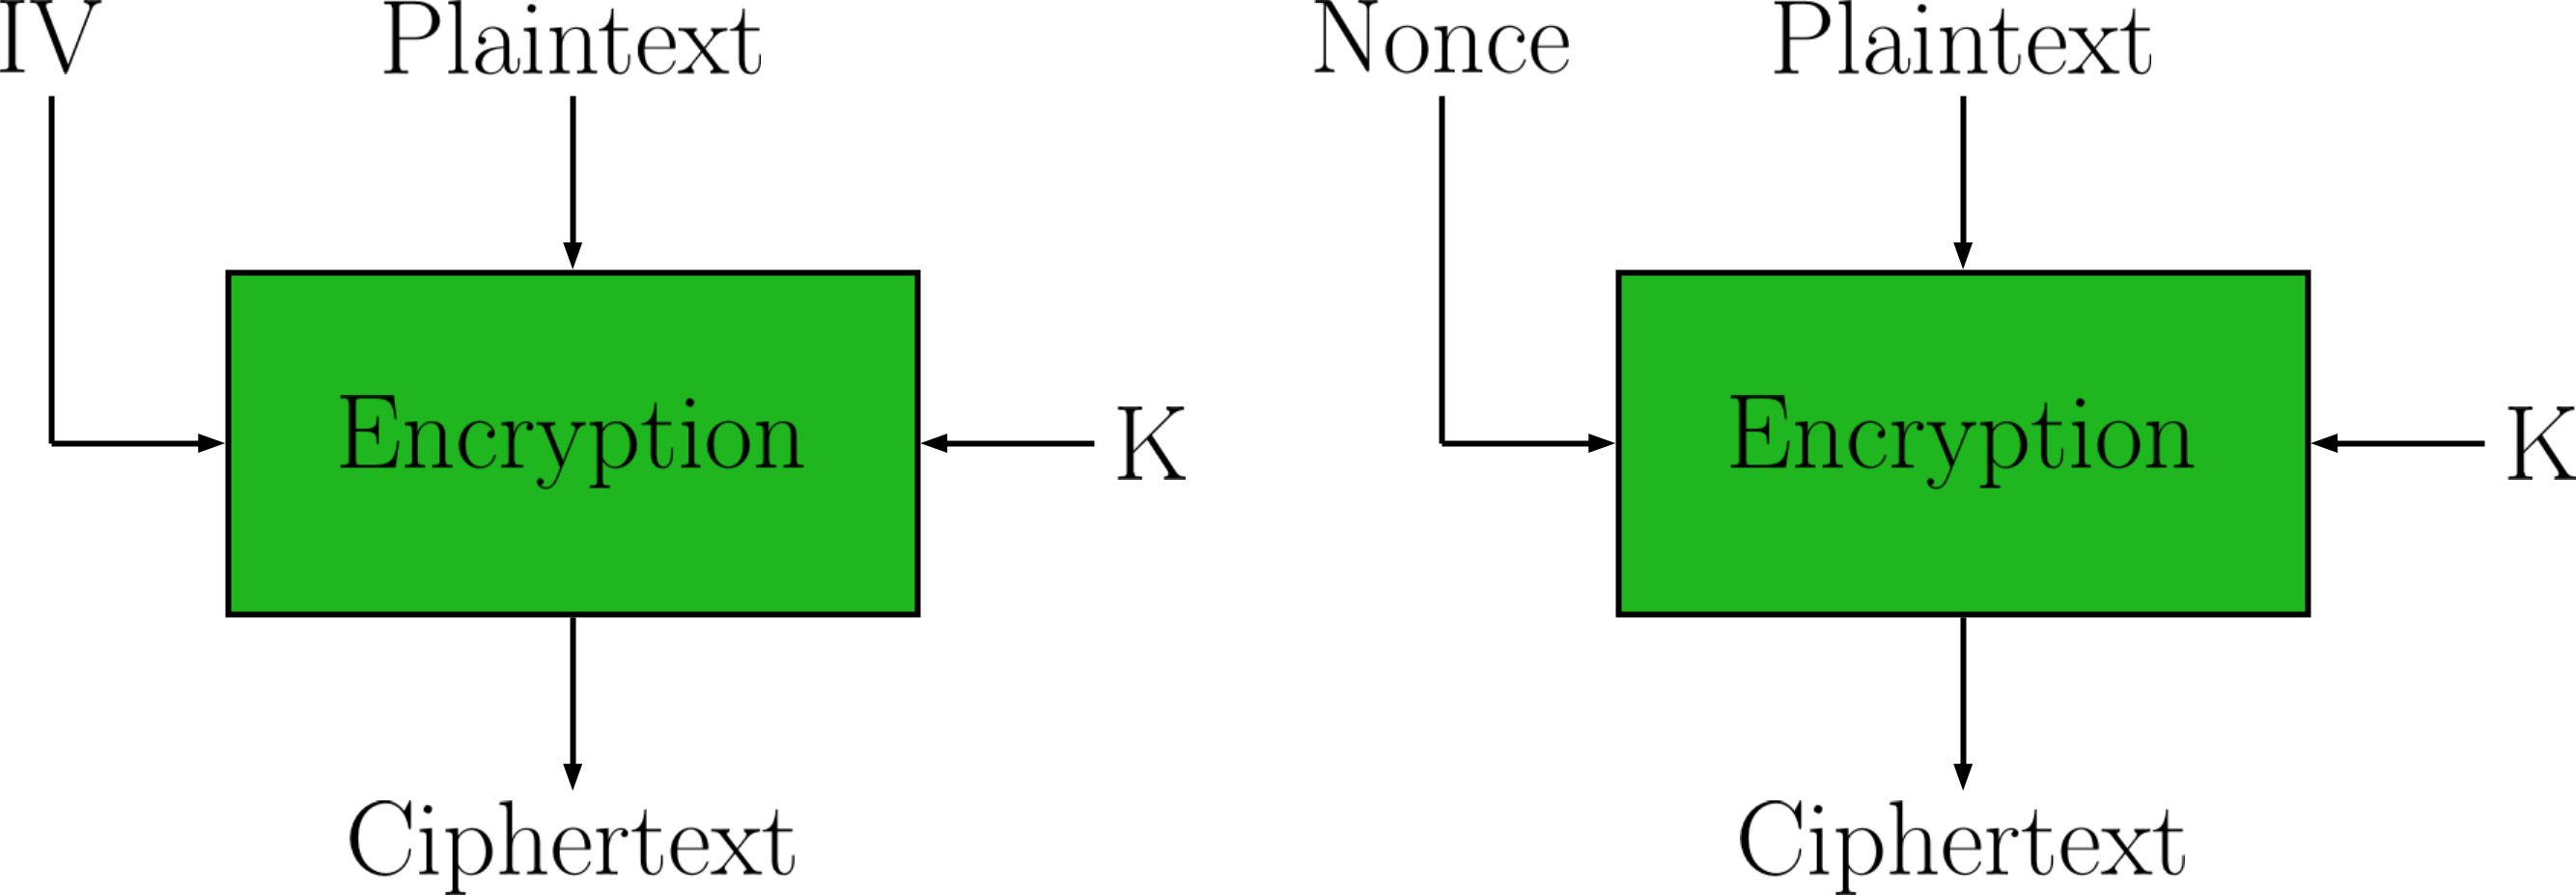
\includegraphics[scale=0.10]{ivnonce.jpg}
\end{center}
\end{frame}

\begin{frame}{Abstraction of the MAC}
To simplify, we can abstract the MAC as a pseudo-random function.
\begin{itemize}
\item vecMAC: A MAC primitive that takes multiple values for its input (here, 3 maximum).
\item strMAC: classic MAC as we know.
\end{itemize}

\begin{center}
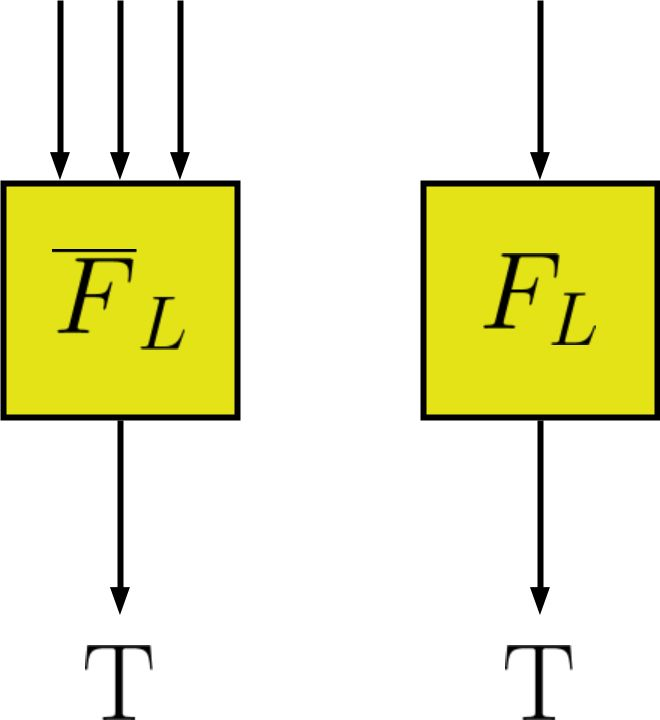
\includegraphics[scale=0.15]{macabstraction.jpg}
\end{center}
\end{frame}

\begin{frame}{Combinations}
Start by creating a basic model and enumerate all possibilities.
There are 160 possible combinations.
\begin{center}
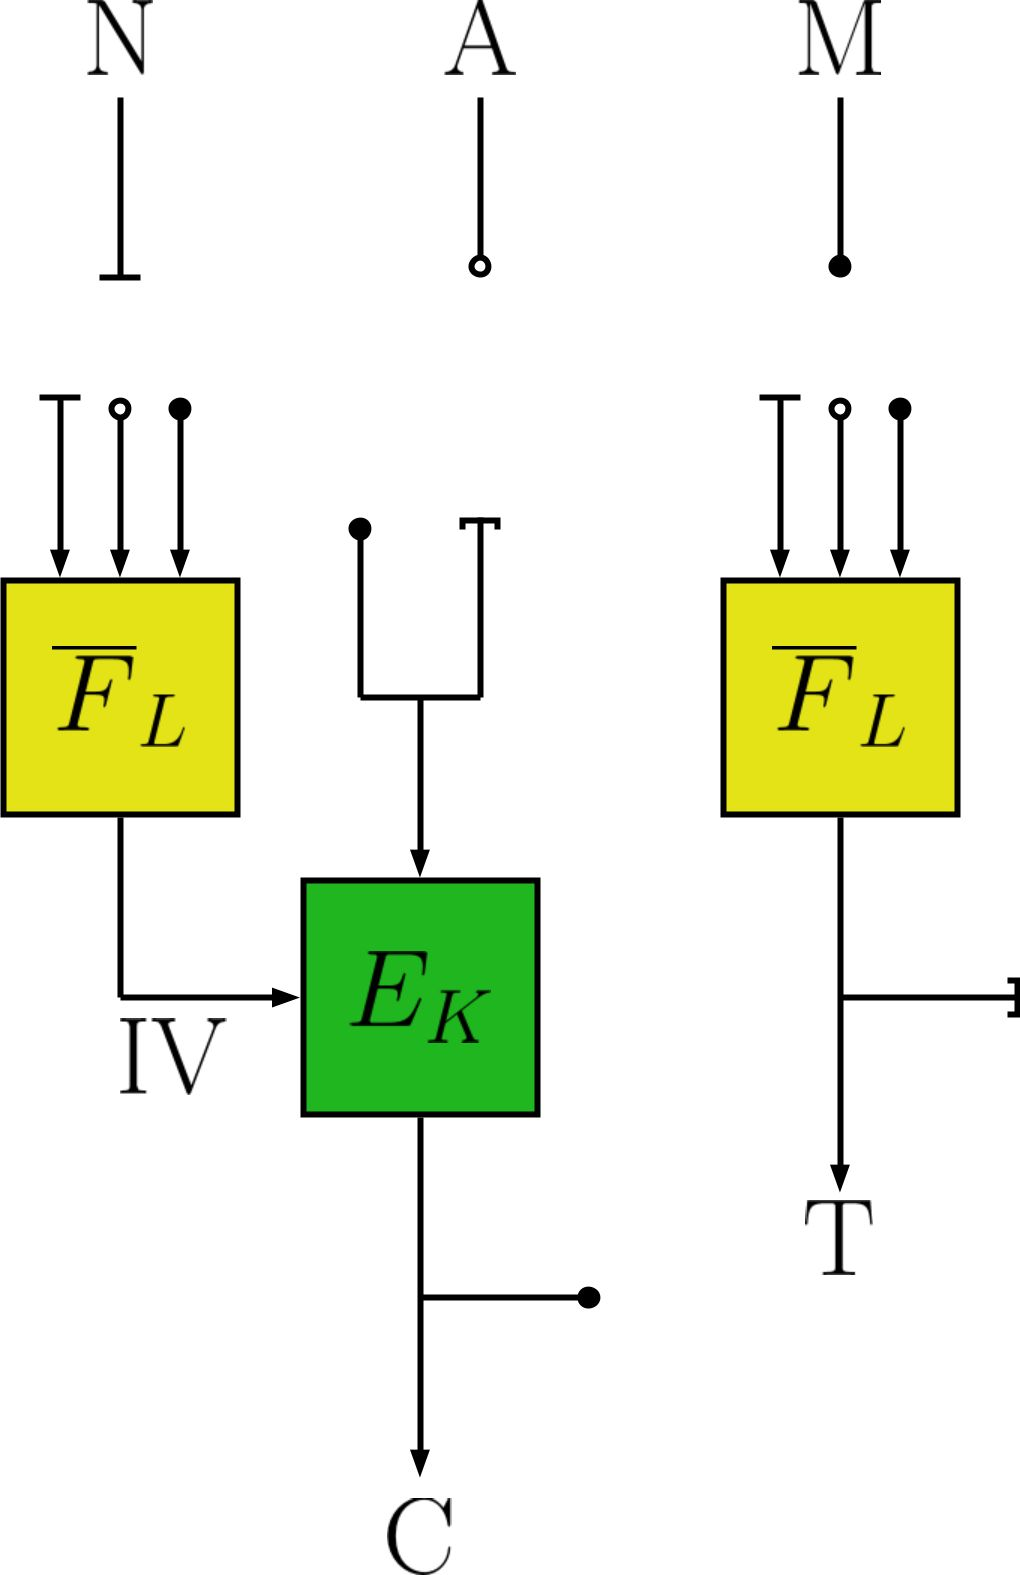
\includegraphics[scale=0.12]{plugs.jpg}
\end{center}
\end{frame}

\begin{frame}{Method}
Eliminate bad schemes by finding trivial attacks.
\begin{center}
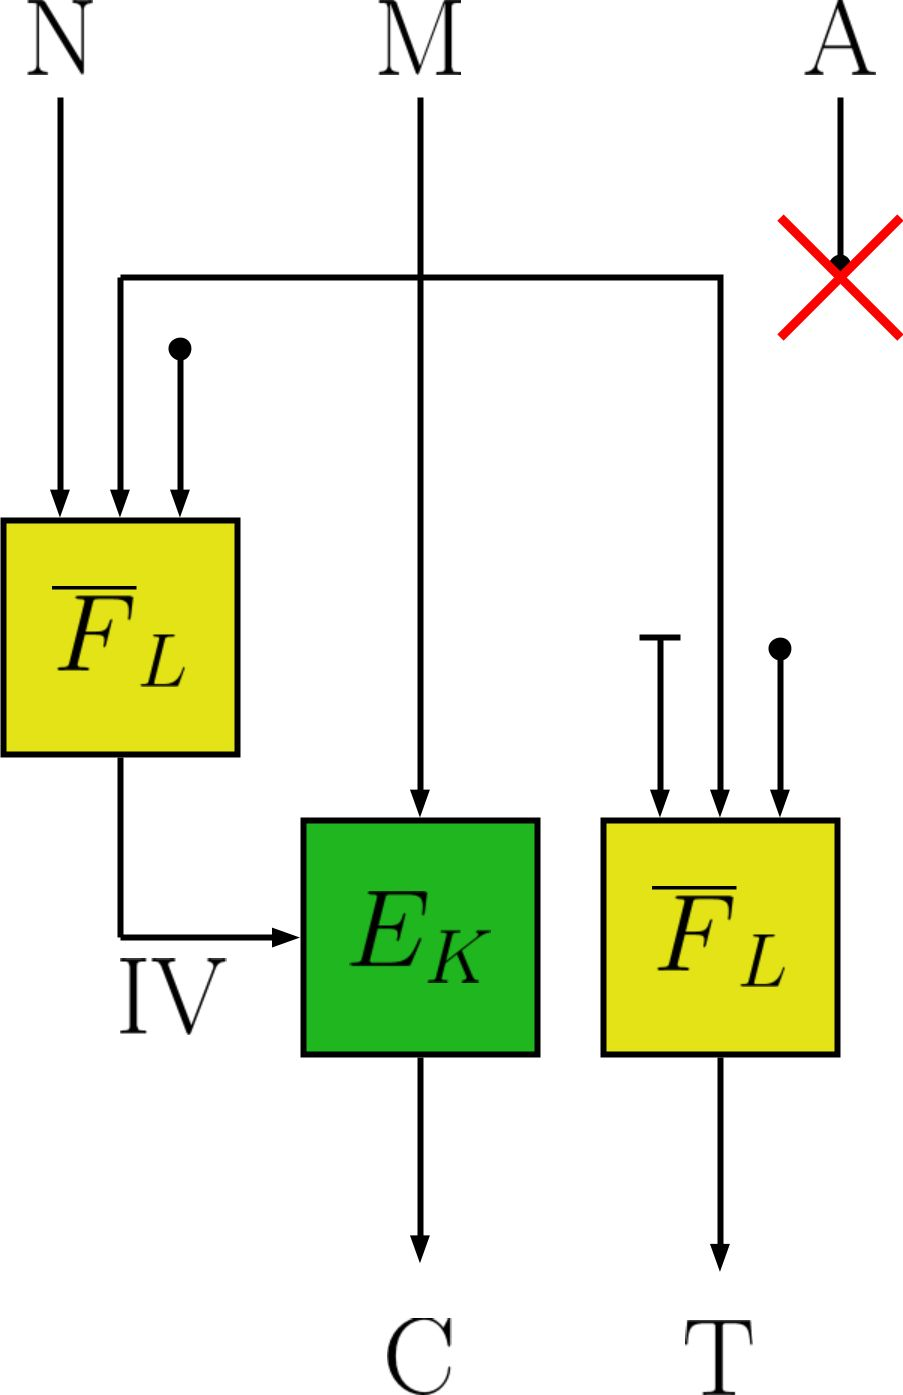
\includegraphics[scale=0.12]{badivae.jpg}
\end{center}
The remaining schemes were analyzed by hand.
\end{frame}

\begin{frame}{A* Schemes}
There were 160 candidates, 8 of them are favored (A1-A8), one has a weaker security bound (A9) and three are elusive (A10-A12).

\begin{tiny}
\begin{center}
\begin{tabular}{ | c | c | c | l | }
        \hline
	Scheme & IV & Tag & Comment \\ \hline
	A1 & $F^{iv}_L(N,\sqcup,\sqcup)$ & $F^{tag}_L(N, A, M)$ & C,T done in parallel \\ \hline
	A2 & $F^{iv}_L(N,A,\sqcup)$ & $F^{tag}_L(N, A, M)$ & C,T done in parallel \\ \hline
	A3 & $F^{iv}_L(N,\sqcup,M)$ & $F^{tag}_L(N, A, M)$ & Assume IV is recoverable, untruncatable \\ \hline
	A4 & $F^{iv}_L(N,A,M)$ & $F^{tag}_L(N, A, M)$ & $F^{iv} = F^{tag}$, untruncatable, nonce-reuse secure \\ \hline
	A5 & $F^{iv}_L(N,\sqcup,\sqcup)$ & $F^{tag}_L(N, A, C)$ & M,T done in parallel \\ \hline
	A6 & $F^{iv}_L(N,A,\sqcup)$ & $F^{tag}_L(N, A, C)$ & M,T done in parallel \\ \hline
	A7 & $F^{iv}_L(N,\sqcup,\sqcup)$ & $F^{tag}_L(N, A, M)$ & Untruncatable \\ \hline
	A8 & $F^{iv}_L(N,A,\sqcup)$ & $F^{tag}_L(N, A, M)$ & Untruncatable \\ \hline
        \hline
	A9 & $F^{iv}_L(N,A,\sqcup)$ & $F^{tag}_L(N, \sqcup, M)$ & Weaker bound, untruncatable \\ \hline
        \hline
	A10 & $F^{iv}_L(N,A,\sqcup)$ & $F^{tag}_L(\sqcup, A, M)$ & Security unresolved \\ \hline
	A11 & $F^{iv}_L(N,A,\sqcup)$ & $F^{tag}_L(\sqcup,\sqcup, M)$ & Security unresolved \\ \hline
	A12 & $F^{iv}_L(N,\sqcup,\sqcup)$ & $F^{tag}_L(\sqcup, A, M)$ & Security unresolved \\ \hline
\end{tabular}
\end{center}
\end{tiny}
\end{frame}

\begin{frame}
\begin{center}
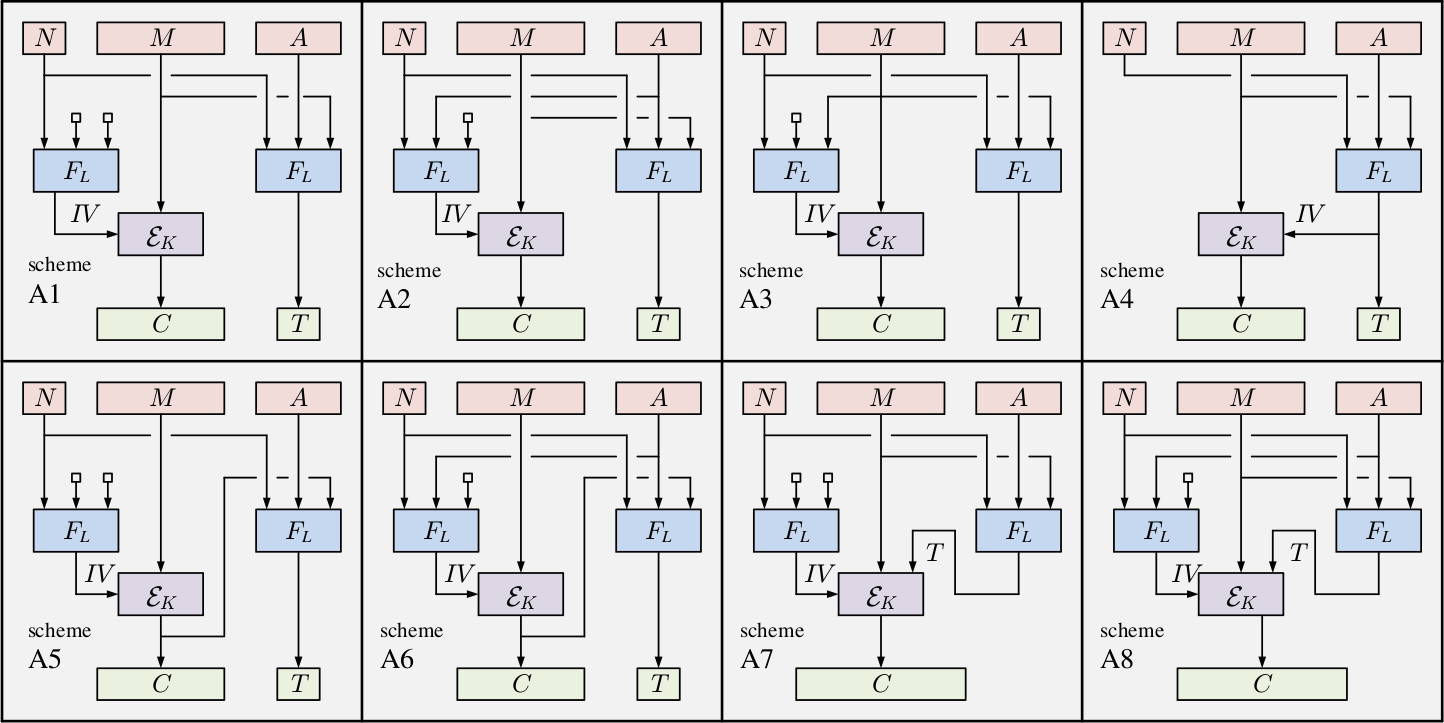
\includegraphics[scale=0.22]{../report/vecmac.jpg}
\end{center}

A1 to A3 is similar to E\&M

A4 is SIV mode.

A5 and A6 is EtM.

A7 and A8 is MtE.
\vfill
{\tiny Image: Namprempre and al., \emph{Reconsidering generic composition}}
\end{frame}

\begin{frame}{From strMAC to vecMAC}
vecMAC is an abstract function, we need something concrete.

Use a \emph{three-xor construction}.

\begin{center}
$F_{L1,L2,L3}(N,A,M) = f^\prime_{L1}(N) \oplus f^\prime_{L2}(A) \oplus f^\prime_{L3}(M)$
\end{center}

This transformation works for the eight A schemes and is proven secure.
We now obtain the B schemes.
\end{frame}

\begin{frame}{B Schemes}
\begin{center}
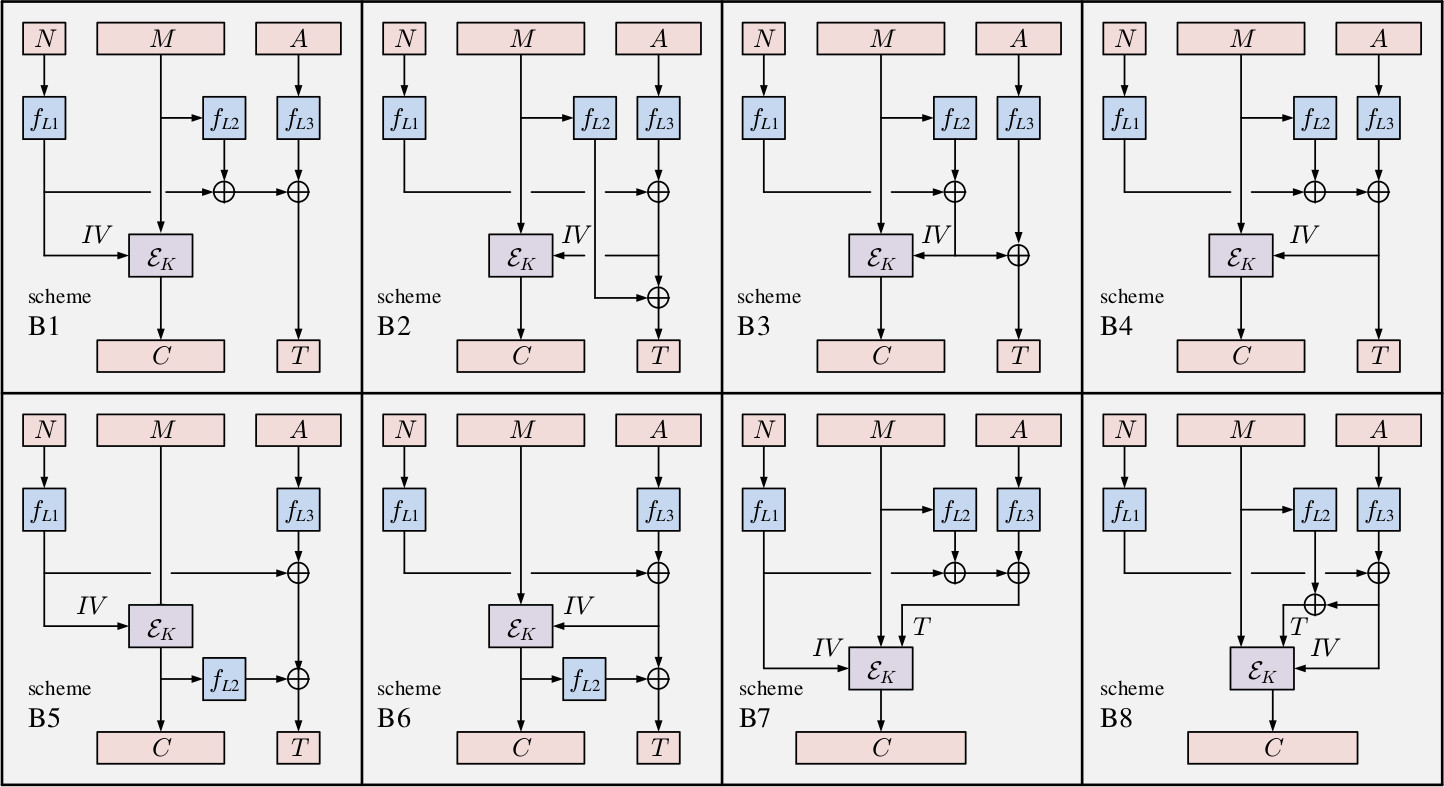
\includegraphics[scale=0.22]{../report/strmac.jpg}
\end{center}

B1 is EAX mode.
\vfill
{\tiny Image: Namprempre and al., \emph{Reconsidering generic composition}}
\end{frame}

\begin{frame}{N Schemes}
Another model with 20 candidates, three are favored and one is elusive.

We can again use the \emph{three-xor construction}, but we keep the simplicity of vecMAC.

\begin{center}
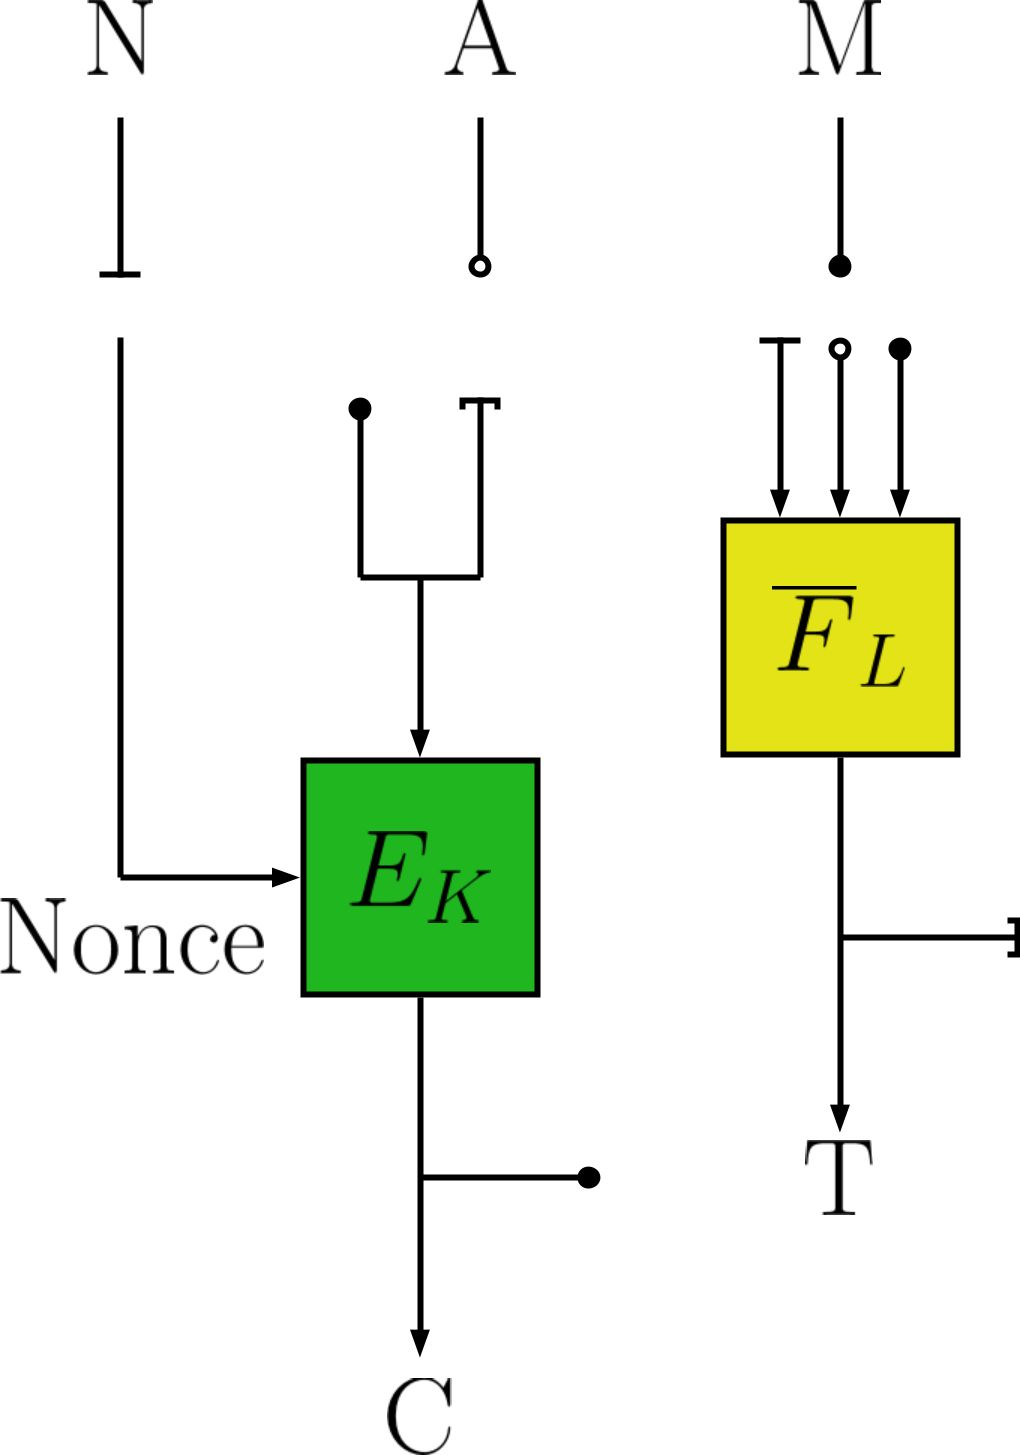
\includegraphics[scale=0.11]{plugsNAE.jpg}
\end{center}
\end{frame}

\begin{frame}{N Schemes}
\begin{center}
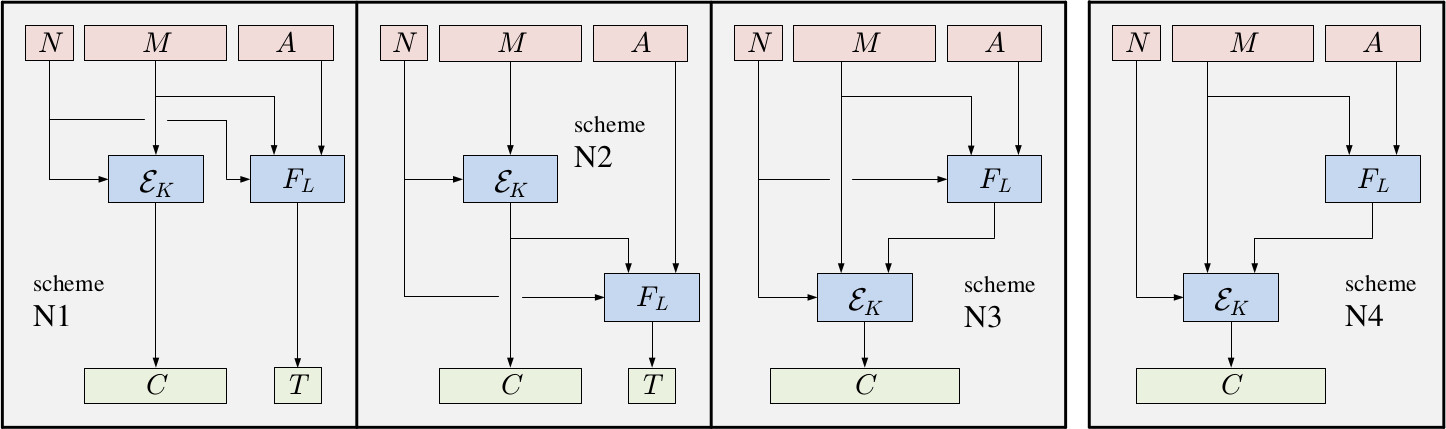
\includegraphics[scale=0.22]{../report/noncemac.jpg}
\end{center}

N1 can compute C and T in parallel.

N2 can compute M and T in parallel.

N3 is untruncatable.

N4 has an unresolved security, and C is untruncatable.
\vfill
{\tiny Image: Namprempre and al., \emph{Reconsidering generic composition}}
\end{frame}

\section{Critique of the ISO 19772 standard}
\begin{frame}{ISO 19772}
Defines GCM, CCM and EAX very well, but EtM is poorly done.
\begin{itemize}
\item Usage of a Starting Value (SV). Unclear if it's a nonce or an IV.
\item SV communication is not specified.
\item What to do in case of a padding error?
\end{itemize}

We do not know if it's a scheme built from a pE, or from an ivE.
\end{frame}

{ % all template changes are local to this group.
    \setbeamertemplate{navigation symbols}{}
    \begin{frame}[plain]
        \begin{tikzpicture}[remember picture,overlay]
            \node[at=(current page.center)] {
                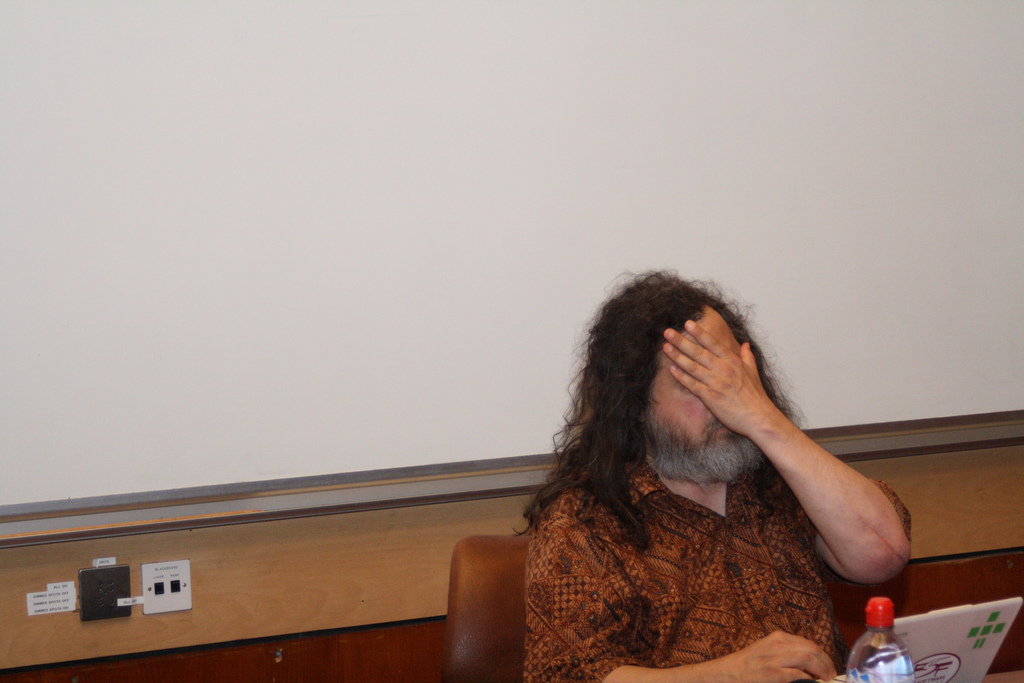
\includegraphics[width=\paperwidth]{stallmanpalm.jpg}
            };
        \end{tikzpicture}
     \end{frame}
}

\section{Conclusion}
\begin{frame}{Conclusion}
\begin{itemize}
\item Be careful when composing with cryptographic primitives. Additivity is not guaranteed.
\item Interpreting cryptography and security results is not trivial. ISO 19772 is a pure example.
\item The new result shown here is more concrete and applicable for real cryptography work.
\end{itemize}
\end{frame}

\begin{frame}
\begin{center}
{\huge Questions and Remarks?}
\end{center}
\end{frame}

\begin{frame}{References}
\begin{tiny}
\begin{thebibliography}{9}
\bibitem{namprempre2014reconsidering}
	Namprempre, Chanathip and Rogaway, Phillip and Shrimpton, Thomas
	\emph{Reconsidering generic composition},
	Annual International Conference on the Theory and Applications of Cryptographic Techniques,
	2014

\bibitem{bellare2000authenticated}
	Bellare, Mihir and Namprempre, Chanathip,
	\emph{Authenticated encryption: Relations among notions and analysis of the generic composition paradigm},
	International Conference on the Theory and Application of Cryptology and Information Security,
	2000

\bibitem{ferguson2010cryptography}
	Ferguson, Niels and Schneier, Bruce and Kohno, Tadayoshi,
	\emph{Cryptography Engineering: Design Principles and Practical Applications},
	Wiley Publishing, Inc.,
	2010

\bibitem{iso197722009}
	ISO/IEC 19772,
	\emph{Information technology - Security techniques - Authenticated encryption},
	2009

\bibitem{stallman}
	Martin Meredith,
	\emph{Facepalm},
	Birmingham, August 25, 2011

\end{thebibliography}
\end{tiny}
\end{frame}

\end{document}
